\subsection{\vdmh}
\Opensolutionfile{ans}[ans/DA-CD3-VD]
\begin{vd}%[2H2N1-2]
\immini[thm]
{
    Hình chóp $S.ABCD$ có đáy $ABCD$ là hình vuông tâm $O$. Hãy chỉ ra mệnh đề \textbf{sai}?
    \choice
    {$\overrightarrow{SA}+\overrightarrow{SC}=2\overrightarrow{SO}$}
    {$\overrightarrow{SB}+\overrightarrow{SD}=2\overrightarrow{SO}$}
    {$\overrightarrow{SA}+\overrightarrow{SC}=\overrightarrow{SB}+\overrightarrow{SD}$}
    {\True $\overrightarrow{SA}+\overrightarrow{SC}+\overrightarrow{SB}+\overrightarrow{SD}=\overrightarrow{0}$}
}
{
    \begin{tikzpicture}[>=stealth,line join=round,line cap=round,font=\small,scale=0.5]
        \path (0,0) coordinate (A)
        (-2.5,-1.4) coordinate (B)
        (6,0) coordinate (D)
        ($(B)+(D)-(A)$) coordinate (C)
        ($(A)!0.5!(C)$) coordinate (O)
        ($(O)+(0.5,6)$)coordinate (S)
        ;
        \draw (S)--(B)--(C)--(S)--(D)--(C);
        \draw[dashed] (O)--(S)--(A)--(B)--(D)--(A)--(C);
        \foreach \d / \g in {A/135,B/-135,C/-45,S/90,O/180,D/45}
        \fill (\d) circle (1.5pt) node[shift={(\g:10pt)}]{$\d$};
    \end{tikzpicture}
}
%    \loigiai{
%        \immini{
%            Ta có $O$ là trung điểm của $AC$ và $BD$ nên
%            $\heva{& \overrightarrow{SA}+\overrightarrow{SC}=2\overrightarrow{SO} \\ & \overrightarrow{SB}+\overrightarrow{SD}=2\overrightarrow{SO}}$\\
%            $\Rightarrow \overrightarrow{SA}+\overrightarrow{SC}=\overrightarrow{SB}+\overrightarrow{SD}$ và
%            $\overrightarrow{SA}+\overrightarrow{SC}+\overrightarrow{SB}+\overrightarrow{SD}=4\overrightarrow{SO}$
%        }{
%            \begin{tikzpicture}[>=stealth,line join=round,line cap=round,font=\small,scale=0.5]
%                \path (0,0) coordinate (A)
%                (-2.5,-1.4) coordinate (B)
%                (6,0) coordinate (D)
%                ($(B)+(D)-(A)$) coordinate (C)
%                ($(A)!0.5!(C)$) coordinate (O)
%                ($(O)+(0.5,6)$)coordinate (S)
%                ;
%                \draw (S)--(B)--(C)--(S)--(D)--(C);
%                \draw[dashed] (O)--(S)--(A)--(B)--(D)--(A)--(C);
%                \foreach \d / \g in {A/135,B/-135,C/-45,S/90,O/180,D/45}
%                \fill (\d) circle (1.5pt) node[shift={(\g:10pt)}]{$\d$};
%    \end{tikzpicture}}}
\end{vd}

\begin{vd}%[2H2N1-2]
    Cho tam giác $ABC$ có trung tuyến $AM$, $(M\in BC)$. Khẳng định sau đây là \textbf{đúng}?
    \choice
    {$\overrightarrow{AM} = -\dfrac{1}{2} \cdot \left( \overrightarrow{AB} + \overrightarrow{AC} \right)$}
    {$\overrightarrow{AM} = \overrightarrow{AB} + 2\overrightarrow{BM}$}
    {$\overrightarrow{AM} =  \dfrac{1}{2} \cdot \left( \overrightarrow{AB} - \overrightarrow{AC} \right)$}
    {\True $\overrightarrow{AM} =  \dfrac{1}{2} \cdot \left( \overrightarrow{AB} + \overrightarrow{AC} \right)$}
%    \loigiai{
%        Vì $AM$ là trung tuyến của $\triangle ABC$ nên ta có $\overrightarrow{AM} =  \dfrac{1}{2} \cdot \left( \overrightarrow{AB} + \overrightarrow{AC} \right)$.
%    }
\dotlineEX{1}
\end{vd}

\begin{vd}%[2H2N1-2]
\immini[thm]
{
    Cho lăng trụ tam giác $ABC.A'B'C'$ có $\overrightarrow{AA'}=\overrightarrow{a}$, $\overrightarrow{AB}=\overrightarrow{b}$, $\overrightarrow{AC}=\overrightarrow{c}$. Hãy phân tích (biểu thị) vectơ $\overrightarrow{BC'}$ qua các vectơ $\overrightarrow{a}$, $\overrightarrow{b}$, $\overrightarrow{c}$
    \choice
    {$\overrightarrow{BC'}=\overrightarrow{a}+\overrightarrow{b}-\overrightarrow{c}$}
    {$\overrightarrow{BC'}=-\overrightarrow{a}+\overrightarrow{b}-\overrightarrow{c}$}
    {$\overrightarrow{BC'}=-\overrightarrow{a}-\overrightarrow{b}+\overrightarrow{c}$}
    {\True $\overrightarrow{BC'}=\overrightarrow{a}-\overrightarrow{b}+\overrightarrow{c}$}
}
{
    \begin{tikzpicture}[scale=0.8,>=stealth,line join=round,line cap=round,font=\small]
        \def\a{4}
        \def\h{4.5}
        \path 	(0:0) coordinate (A)
        ++(0:\a) coordinate (C)
        ++(-150:3*\a/4) coordinate (B)
        ($(A)+(80:\h)$) coordinate (A')
        ($(B)+(80:\h)$) coordinate (B')
        ($(C)+(80:\h)$) coordinate (C');
        \draw[dashed,thick] 	(A)--(C)node[midway, above]{$\overrightarrow{c}$};
        \draw[thick]	(C)--(C') 	(B)--(B')	(A)--(A')node[midway, left]{$\overrightarrow{a}$} (A)--(B)node[midway, left]{$\overrightarrow{b}$}  (B)--(C) (A')--(B')--(C')--cycle;
        \foreach \d / \g in {A/180,B/-45,C/0,A'/180,B'/-45,C'/0}
        \fill (\d) circle (1.5pt) node[shift={(\g:10pt)}]{$\d$};
    \end{tikzpicture}
}
%    \loigiai{\;
%        \begin{center}
%            \begin{tikzpicture}[scale=0.8,>=stealth,line join=round,line cap=round,font=\small]
%                \def\a{4}
%                \def\h{4.5}
%                \path 	(0:0) coordinate (A)
%                ++(0:\a) coordinate (C)
%                ++(-150:3*\a/4) coordinate (B)
%                ($(A)+(80:\h)$) coordinate (A')
%                ($(B)+(80:\h)$) coordinate (B')
%                ($(C)+(80:\h)$) coordinate (C');
%                \draw[dashed,thick] 	(A)--(C)node[midway, above]{$\overrightarrow{c}$};
%                \draw[thick]	(C)--(C') 	(B)--(B')	(A)--(A')node[midway, left]{$\overrightarrow{a}$} (A)--(B)node[midway, left]{$\overrightarrow{b}$}  (B)--(C) (A')--(B')--(C')--cycle;
%                \foreach \d / \g in {A/180,B/-45,C/0,A'/180,B'/-45,C'/0}
%                \fill (\d) circle (1.5pt) node[shift={(\g:10pt)}]{$\d$};
%            \end{tikzpicture}
%        \end{center}
%        $\overrightarrow{BC'}=\overrightarrow{BC}+\overrightarrow{CC'}=\overrightarrow{BA}+\overrightarrow{AC}+\overrightarrow{CC'}=\overrightarrow{AA'}-\overrightarrow{AB}+\overrightarrow{AC}=\overrightarrow{a}-\overrightarrow{b}+\overrightarrow{c}$.}
\end{vd}

\begin{vd}%[2H2H1-2]
\immini[thm]
{
    Cho hình lăng trụ tam giác $ABC.A'B'C'$. Đặt $\overrightarrow{AA'}=\overrightarrow{a}$, $\overrightarrow{AB}=\overrightarrow{b}$, $\overrightarrow{AC}=\overrightarrow{c}$, $\overrightarrow{BC}=\overrightarrow{d}$. Trong các biểu thức vec tơ sau đây, biểu thức nào là đúng?
    \choice
    {$\overrightarrow{a}=\overrightarrow{b}+\overrightarrow{c}$}
    {$\overrightarrow{a}+\overrightarrow{b}+\overrightarrow{c}+\overrightarrow{d}=\overrightarrow{0}$}
    {\True $\overrightarrow{b}-\overrightarrow{c}+\overrightarrow{d}=\overrightarrow{0}$}
    {$\overrightarrow{a}+\overrightarrow{b}+\overrightarrow{c}=\overrightarrow{d}$}
}
{
    \begin{tikzpicture}[scale=1, font=\small, line join=round, line cap=round, >=stealth]
        \def\a{4}
        \def\h{4.5}
        \path (0:0) coordinate (A)
        ++(0:\a) coordinate (C)
        ++(-150:3*\a/4) coordinate (B)
        ($(A)+(100:\h)$) coordinate (A')
        ($(B)+(100:\h)$) coordinate (B')
        ($(C)+(100:\h)$) coordinate (C');
        \draw[dashed] (A)--(C);
        \draw (C)--(C') (B)--(B') (A)--(A') (A)--(B)--(C) (A')--(B')--(C')--cycle;
        \foreach \d / \g in {A/180,B/-45,C/0,A'/180,B'/-45,C'/0}
        \fill (\d) circle (1.5pt) node[shift={(\g:10pt)}]{$\d$};
    \end{tikzpicture}
}
%    \loigiai{
%        \begin{center}
%            \begin{tikzpicture}[scale=1, font=\small, line join=round, line cap=round, >=stealth]
%                \def\a{4}
%                \def\h{4.5}
%                \path (0:0) coordinate (A)
%                ++(0:\a) coordinate (C)
%                ++(-150:3*\a/4) coordinate (B)
%                ($(A)+(100:\h)$) coordinate (A')
%                ($(B)+(100:\h)$) coordinate (B')
%                ($(C)+(100:\h)$) coordinate (C');
%                \draw[dashed] (A)--(C);
%                \draw (C)--(C') (B)--(B') (A)--(A') (A)--(B)--(C) (A')--(B')--(C')--cycle;
%                \foreach \d / \g in {A/180,B/-45,C/0,A'/180,B'/-45,C'/0}
%                \fill (\d) circle (1.5pt) node[shift={(\g:10pt)}]{$\d$};
%            \end{tikzpicture}
%        \end{center}
%        Ta có $\overrightarrow{b}-\overrightarrow{c}+\overrightarrow{d}=\overrightarrow{AB}-\overrightarrow{AC}+\overrightarrow{BC}=\overrightarrow{CB}+\overrightarrow{BC}=\overrightarrow{0}$.
%    }
\end{vd}

\begin{vd}%[2H2H1-2]
    \immini[thm]{Cho lập phương $ABCD.A'B'C'D'$ có độ dài mỗi cạnh bằng $1$. Tính độ dài của vectơ $\overrightarrow{AC}+\overrightarrow{C'D'}$.
     \choice
        {$\sqrt{3}$}
        {$\sqrt{2}$}
        {\True $1$}
        {$2\sqrt{2}$}}
    {
        \begin{tikzpicture}[scale=1, font=\small, line join=round, line cap=round, >=stealth]
            \def\a{3}
            \def\b{2}
            \def\h{3}
            \path (0:0) coordinate (A)
            ++(0:\a) coordinate (D)
            ++(-130:\b) coordinate (C)
            ($(A)+(C)-(D)$) coordinate (B)
            ($(A)+(90:\h)$) coordinate (A')
            ($(B)+(90:\h)$) coordinate (B')
            ($(C)+(90:\h)$) coordinate (C')
            ($(D)+(90:\h)$) coordinate (D');
            \draw[dashed] (B)--(A)--(D) (A)--(A') (A)--(C);
            \draw (C)--(C') (D)--(D') (B)--(B') (C)--(C')--(A')
            (B)--(C)--(D)
            (A')--(B')--(C')--(D')--cycle;
            \foreach \d / \g in {A/180,B/180,C/0,D/0,A'/180,B'/180,C'/0,D'/0}
            \fill (\d) circle (1.5pt) node[shift={(\g:10pt)}]{$\d$};
        \end{tikzpicture}
    }
%    \loigiai{
%        Ta có: $A'C'CA$ là hình chữ nhật nên $\overrightarrow{A'C'}=\overrightarrow{AC}$.\\
%        Khi đó, $\overrightarrow{AC}+\overrightarrow{C'D'}=\overrightarrow{A'C'}+\overrightarrow{C'D'}=\overrightarrow{A'D'}$.\\
%        Vậy $\left|\overrightarrow{AC}+\overrightarrow{C'D'}\right|=\left|\overrightarrow{A'D'}\right|=A'D'=1$.
%    }
\end{vd}

\begin{vd}%[2H2H1-2]
\immini[thm]
{
    Cho tứ diện $ABCD$. Khẳng định nào sau đây là đúng?
    \choice
    {$\overrightarrow{AB} - \overrightarrow{CD} =\overrightarrow{AD} - \overrightarrow{BC}$}
    {\True $\overrightarrow{AB} + \overrightarrow{CD} =\overrightarrow{AD} + \overrightarrow{CB}$}
    {$\overrightarrow{AB} + \overrightarrow{CD} =\overrightarrow{AD} + \overrightarrow{BC}$}
    {$\overrightarrow{AB} + \overrightarrow{CD} =\overrightarrow{AC} + \overrightarrow{BD}$}
}
{
    \begin{tikzpicture}[scale=1, font=\small, line join=round, line cap=round, >=stealth]
        \def\h{3}
        \path (0,0) coordinate (B)
        (1.3,-1.2) coordinate (C)
        (4,0) coordinate (D)
        (1,\h) coordinate(A)
        ($(B)!1/2!(D)$) coordinate(M);
        \draw (A)--(B)--(C)--(D)--(A)--(C);
        \draw[dashed] (B)--(D) (C)--(M);
        \foreach \d/\g in {A/90, B/180, C/-90, D/0, M/70} \fill (\d) circle (1.5pt) node[shift={(\g:10pt)}]{$\d$};;
    \end{tikzpicture}
}
%    \loigiai
%    {\begin{center}
%            \begin{tikzpicture}[scale=1, font=\small, line join=round, line cap=round, >=stealth]
%                \def\h{3}
%                \path (0,0) coordinate (B)
%                (1.3,-1.2) coordinate (C)
%                (4,0) coordinate (D)
%                (1,\h) coordinate(A)
%                ($(B)!1/2!(D)$) coordinate(M);
%                \draw (A)--(B)--(C)--(D)--(A)--(C);
%                \draw[dashed] (B)--(D) (C)--(M);
%                \foreach \d/\g in {A/90, B/180, C/-90, D/0, M/70} \fill (\d) circle (1.5pt) node[shift={(\g:10pt)}]{$\d$};;
%            \end{tikzpicture}
%        \end{center}
%        \begin{itemize}
%            \item Ta có $\overrightarrow{AB} + \overrightarrow{CD} = \left(\overrightarrow{AD} + \overrightarrow{DB}\right) + \overrightarrow{CD} = \overrightarrow{AD} + \left(\overrightarrow{CD} + \overrightarrow{DB}\right) = \overrightarrow{AD} + \overrightarrow{CB}$.
%            \item Vì $\overrightarrow{BC}\neq \overrightarrow{0}$ nên khẳng định $\overrightarrow{AB} + \overrightarrow{CD} =\overrightarrow{AD} + \overrightarrow{BC}$ là sai.
%            \item Nếu $\overrightarrow{AB} - \overrightarrow{CD} =\overrightarrow{AD} - \overrightarrow{BC} \Leftrightarrow \overrightarrow{AB} - \overrightarrow{AD} = \overrightarrow{CB} + \overrightarrow{CD} \Leftrightarrow \overrightarrow{DB} = 2\overrightarrow{CM}$ (với $M$ là trung điểm của $BD$), suy ra $B$, $D$, $M$, $C$ thẳng hàng. Điều này vô lý nên khẳng định $\overrightarrow{AB} - \overrightarrow{CD} =\overrightarrow{AD} - \overrightarrow{BC}$ là sai.
%            \item Nếu $\overrightarrow{AB} + \overrightarrow{CD} =\overrightarrow{AC} + \overrightarrow{BD} \Leftrightarrow \overrightarrow{AB} - \overrightarrow{AC} = \overrightarrow{DC} - \overrightarrow{DB} \Leftrightarrow \overrightarrow{CB} = \overrightarrow{BC}$, điều này vô lý nên khẳng định $\overrightarrow{AB} + \overrightarrow{CD} =\overrightarrow{AC} + \overrightarrow{BD}$ là sai.
%    \end{itemize}}
\end{vd}

\begin{vd}%[2H2H1-2]
\immini[thm]
{
    Cho tứ diện $ABCD$ biết $AB=BC=CA=4=AD=4$, $DC=6$, $BD=7$ và $\triangle ABC$, $\triangle DBC$ nằm trên hai mặt phẳng vuông góc. Tính $\left|\overrightarrow{DA}+\overrightarrow{DI}\right|$ với $I$ là trung điểm $BC$.
    \choice
    {\True $\sqrt{97}$}
    {$\dfrac{\sqrt{97}}{4}$}
    {$\dfrac{97}{4}$}
    {$\dfrac{\sqrt{97}}{2}$}
}
{
    \begin{tikzpicture}[scale=1, font=\small, line join=round, line cap=round, >=stealth]
        \coordinate (D) at (0, 0);
        \coordinate (C) at (2, -1);
        \coordinate (B) at (5, 0.2);
        \coordinate (I) at ($(B)!0.5!(C)$);
        \coordinate (A) at ($(I)+(0,4)$);
        \coordinate (M) at ($(A)!0.5!(I)$);
        \draw (C) -- (A) -- (B) -- (C) -- (D) -- (A) -- (I);
        \draw[dashed] (M) -- (D) -- (I) (D) -- (B) ;
        %\pic[draw,thin,angle radius=2mm] {right angle = S--A--C} pic[draw,thin,angle radius=2mm] {right angle = A--B--C} pic[draw,thin,angle radius=2mm] {right angle = A--H--B};
        \foreach \d/\g in {A/90,B/0,D/180,C/-90,I/-90,M/0}{\fill (\d) circle (1.5pt) node[shift={(\g:10pt)}]{$\d$};}
    \end{tikzpicture}
}
%    \loigiai{
%        \begin{center}
%            \begin{tikzpicture}[scale=1, font=\small, line join=round, line cap=round, >=stealth]
%                \coordinate (D) at (0, 0);
%                \coordinate (C) at (2, -1);
%                \coordinate (B) at (5, 0.2);
%                \coordinate (I) at ($(B)!0.5!(C)$);
%                \coordinate (A) at ($(I)+(0,4)$);
%                \coordinate (M) at ($(A)!0.5!(I)$);
%                \draw (C) -- (A) -- (B) -- (C) -- (D) -- (A) -- (I);
%                \draw[dashed] (M) -- (D) -- (I) (D) -- (B) ;
%                %\pic[draw,thin,angle radius=2mm] {right angle = S--A--C} pic[draw,thin,angle radius=2mm] {right angle = A--B--C} pic[draw,thin,angle radius=2mm] {right angle = A--H--B};
%                \foreach \d/\g in {A/90,B/0,D/180,C/-90,I/-90,M/0}{\fill (\d) circle (1.5pt) node[shift={(\g:10pt)}]{$\d$};}
%            \end{tikzpicture}
%        \end{center}
%        Vì $AB=AC=BC=4\Rightarrow \triangle ABC$ đều, I là trung điểm $BC\Rightarrow AI\perp BC$.\\
%        Mặt phẳng $\left(ABC\right)$ và $\left(BCD\right)$ vuông góc với nhau $\Rightarrow AI\perp \left(BCD\right)$.\\
%        Gọi $M$ là trung điểm $AI$.\\
%        Theo quy tắc hình bình hành ta có $\overrightarrow{DI}+\overrightarrow{DA}=2\overrightarrow{DM}\Rightarrow \left|\overrightarrow{DI}+\overrightarrow{DA}\right|=2\cdot\left|\overrightarrow{DM}\right|=2DM$.\\
%        $AI$ là đường cao trong tam giác đều $ABC\Rightarrow AI=2\sqrt{3}$.\\
%        trong tam giác $DBC$ có $DI$ là đường trung tuyến
%        $$DI^2=\dfrac{BD^2}{2}+\dfrac{DC^2}{2}-\dfrac{BC^2}{4}=\dfrac{7^2+6^2}{2}-\dfrac{4^2}{4}=38,5.$$
%        Trong tam giác $ADI$ có $DM$ là đường trung tuyến
%        $$ DM^2=\dfrac{DI^2+AD^2}{2}-\dfrac{AI^2}{4}=\dfrac{38,5+4^2}{2}-\dfrac{(2\sqrt{3})^2}{4}=\dfrac{97}{4} \Rightarrow DM=\dfrac{\sqrt{97}}{2}.$$
%        Vậy $\left|\overrightarrow{DA}+\overrightarrow{DI}\right|=\sqrt{97}.$
%    }
\dotlineEX{1}
\end{vd}
\begin{vd}%[2H2H1-3]
    \immini[thm]
{
    Cho tứ diện $SABC$ có $SA=SB=SC=AB=AC=a$,$BC=a\sqrt{2}$. Tích vô hướng $\overrightarrow{SA}\cdot\overrightarrow{AB}$ bằng
        \choice
        {$a^2$}
        {\True $-\dfrac{a^2}{2}$}
        {$\dfrac{a^2}{2}$}
        {$-a^2$}
    }
    {
        \begin{tikzpicture}[scale=1, font=\small,>=stealth,font=\small,line cap=round,line join=round]
            \def\canhAC{4};\def\canhBA{2};\def\gocBAC{-50};\def\h{3};\def\xdinhS{1};
            %Gán tọa độ.
            \coordinate (A) at (0,0);
            \coordinate (B) at ($(A)+(\gocBAC:\canhBA)$);
            \coordinate (C) at ($(A)+(0:\canhAC)$);
            \coordinate (S) at ($(A)+(\xdinhS,\h)$);
            %Vẽ khối chóp S.ABC.
            \draw (S)--(B) (S)--(A)--(B) (S)--(C)--(B);
            \draw[dashed] (A)--(C);
            %Gán nhãn.
            \foreach \d/\g in {S/90,A/180,B/-90,C/0}{\fill (\d) circle (1.5pt) node[shift={(\g:10pt)}]{$\d$};}
        \end{tikzpicture}
    }
%    \loigiai{
%        \immini{Vì $\triangle SAB$ là tam giác đều nên
%            \allowdisplaybreaks
%            \begin{eqnarray*}
%                \overrightarrow{SA}\cdot\overrightarrow{AB}&=&-\overrightarrow{AS}\cdot\overrightarrow{AB}\\
%                &=&-|\overrightarrow{AS}|\cdot|\overrightarrow{AB}|\cdot\cos\widehat{SAB}\\
%                &=&-a\cdot a\cdot\cos60^\circ\\
%                &=&-\dfrac{a^2}{2}.
%            \end{eqnarray*}
%        }{
%            \begin{tikzpicture}[scale=1, font=\small,>=stealth,font=\small,line cap=round,line join=round]
%                \def\canhAC{4};\def\canhBA{2};\def\gocBAC{-50};\def\h{3};\def\xdinhS{1};
%                %Gán tọa độ.
%                \coordinate (A) at (0,0);
%                \coordinate (B) at ($(A)+(\gocBAC:\canhBA)$);
%                \coordinate (C) at ($(A)+(0:\canhAC)$);
%                \coordinate (S) at ($(A)+(\xdinhS,\h)$);
%                %Vẽ khối chóp S.ABC.
%                \draw (S)--(B) (S)--(A)--(B) (S)--(C)--(B);
%                \draw[dashed] (A)--(C);
%                %Gán nhãn.
%                \foreach \d/\g in {S/90,A/180,B/-90,C/0}{\fill (\d) circle (1.5pt) node[shift={(\g:10pt)}]{$\d$};}
%            \end{tikzpicture}
%        }
%    }

\end{vd}
\begin{vd}%[2H2H1-3]
\immini[thm]
{
    Cho hình lập phương $ABCD.A'B'C'D'$ cạnh bằng $a$. Tích vô hướng của hai vectơ $\overrightarrow{DD'}$ và $\overrightarrow{A'C'}$ bằng
    \choice
    {$\sqrt{2}a^2$}
    {$a^2$}
    {$-\sqrt{2}a^2$}
    {\True $0$}
}
{
    \begin{tikzpicture}
        \def\a{3.5}
        \path (0:0) coordinate (A)
        ++(0:\a) coordinate (D)
        ++(-130:\a/2) coordinate (C)
        ($(A)+(C)-(D)$) coordinate (B)
        ($(A)+(90:\a)$) coordinate (A')
        ($(B)+(90:\a)$) coordinate (B')
        ($(C)+(90:\a)$) coordinate (C')
        ($(D)+(90:\a)$) coordinate (D');
        \draw[dashed] (B)--(A)--(D) (A)--(A');
        \draw (C)--(C')--(A') (D)--(D') (B)--(B') (B)--(C)--(D) (A')--(B')--(C')--(D')--cycle;
        \foreach \d/\g in {A/180,B/180,C/0,D/0,A'/180,B'/180,C'/0,D'/0}
        \fill (\d) circle (1.5pt) node[shift={(\g:10pt)}]{$\d$};
    \end{tikzpicture}
}
%    \loigiai{
%        \begin{center}
%            \begin{tikzpicture}
%                \def\a{3.5}
%                \path (0:0) coordinate (A)
%                ++(0:\a) coordinate (D)
%                ++(-130:\a/2) coordinate (C)
%                ($(A)+(C)-(D)$) coordinate (B)
%                ($(A)+(90:\a)$) coordinate (A')
%                ($(B)+(90:\a)$) coordinate (B')
%                ($(C)+(90:\a)$) coordinate (C')
%                ($(D)+(90:\a)$) coordinate (D');
%                \draw[dashed] (B)--(A)--(D) (A)--(A');
%                \draw (C)--(C')--(A') (D)--(D') (B)--(B') (B)--(C)--(D) (A')--(B')--(C')--(D')--cycle;
%                \foreach \d/\g in {A/180,B/180,C/0,D/0,A'/180,B'/180,C'/0,D'/0}
%                \fill (\d) circle (1.5pt) node[shift={(\g:10pt)}]{$\d$};
%            \end{tikzpicture}
%        \end{center}
%        Ta có $\overrightarrow{A'C'}=\overrightarrow{A'D'}+\overrightarrow{D'C'}$, mà tứ giác $ADD'A'$ và $DCC'D'$ là hình vuông nên
%        $$\overrightarrow{DD'}\cdot \overrightarrow{A'D'}=\overrightarrow{DD'}\cdot \overrightarrow{D'C'}=0.$$
%        Do đó $\overrightarrow{DD'}\cdot\left(\overrightarrow{A'D'}+\overrightarrow{D'C'}\right)=0$.
%    }
\dotlineEX{1}
\end{vd}



\begin{vd}%[2-H2B1-SO-1-2425]%[VN-MT-7, Huỳnh Thanh Chí]%[2H2H1-3]
\immini[thm]
{
    Cho hình hộp $ABCD.A'B'C'D'$. Đẳng thức sau đây là {\bf sai}?
    \choice
    {$\overrightarrow{AC'}=\overrightarrow{AB}+\overrightarrow{AD}+\overrightarrow{AA'}$}
    {$\overrightarrow{AB}=\overrightarrow{D'C'}$}
    {\True $\overrightarrow{AB}+\overrightarrow{AA'}=\overrightarrow{AD}+\overrightarrow{DD'}$}
    {$\overrightarrow{AD}+\overrightarrow{DC}+\overrightarrow{CC'}=\overrightarrow{AD'}+\overrightarrow{D'C'}$}
}
{
    \begin{tikzpicture}[scale=0.9,font=\small,line join=round,line cap=round,>=stealth]
        \def\a{3.5}
        \def\h{4}
        \path (0:0) coordinate (A)
        ++(0:\a) coordinate (D)
        ++(-130:\a/2) coordinate (C)
        ($(A)+(C)-(D)$) coordinate (B)
        ($(A)!0.25!(C)$) coordinate (H)
        ($(H)+(90:\h)$) coordinate (A')
        ($(A')+(C)-(A)$) coordinate (C')
        ($(C')+(B)-(C)$) coordinate (B')
        ($(A')+(D)-(A)$) coordinate (D')
        ($(A)!0.5!(C)$) coordinate (O)
        ;
        \draw[dashed] (B)--(A)--(D) (A)--(A');
        \draw (C)--(C') (D)--(D') (B)--(B') (B)--(C)--(D) (A')--(B')--(C')--(D')--cycle;
        \foreach \d/\g in {A/180,B/180,C/0,D/0,A'/180,B'/180,C'/0,D'/0}
        \fill (\d) circle (1.5pt) node[shift={(\g:10pt)}]{$\d$};
        % \draw pic[draw,angle radius=2mm]{right angle=A'--H--C};%Theo chiều dương
    \end{tikzpicture}
}
%    \loigiai{
%        \begin{center}
%            \begin{tikzpicture}[scale=0.9,font=\small,line join=round,line cap=round,>=stealth]
%                \def\a{3.5}
%                \def\h{4}
%                \path (0:0) coordinate (A)
%                ++(0:\a) coordinate (D)
%                ++(-130:\a/2) coordinate (C)
%                ($(A)+(C)-(D)$) coordinate (B)
%                ($(A)!0.25!(C)$) coordinate (H)
%                ($(H)+(90:\h)$) coordinate (A')
%                ($(A')+(C)-(A)$) coordinate (C')
%                ($(C')+(B)-(C)$) coordinate (B')
%                ($(A')+(D)-(A)$) coordinate (D')
%                ($(A)!0.5!(C)$) coordinate (O)
%                ;
%                \draw[dashed] (B)--(A)--(D) (A)--(A');
%                \draw (C)--(C') (D)--(D') (B)--(B') (B)--(C)--(D) (A')--(B')--(C')--(D')--cycle;
%                \foreach \d/\g in {A/180,B/180,C/0,D/0,A'/180,B'/180,C'/0,D'/0}
%                \fill (\d) circle (1.5pt) node[shift={(\g:10pt)}]{$\d$};
%                % \draw pic[draw,angle radius=2mm]{right angle=A'--H--C};%Theo chiều dương
%            \end{tikzpicture}
%        \end{center}
%        Xét đẳng thức $\overrightarrow{AB}+\overrightarrow{AA'}=\overrightarrow{AD}+\overrightarrow{DD'}$ mà $\overrightarrow{AA'}=\overrightarrow{DD'}$ suy ra $\overrightarrow{AB}=\overrightarrow{AD}$ (sai).\\
%        Do đó, đẳng thức $\overrightarrow{AB}+\overrightarrow{AA'}=\overrightarrow{AD}+\overrightarrow{DD'}$ sai.
%    }
    \dotlineEX{4}
\end{vd}



\begin{vd}%[2H2H1-3]
\immini[thm]
{
    Cho tứ diện đều $ABCD$ cạnh bằng $1$. Giá trị của biểu thức $S = \left| \overrightarrow{AB} + \overrightarrow{AC} + \overrightarrow{AD} \right|$ bằng
    \choice
    {$\dfrac{\sqrt{6}}{2}$}
    {$\sqrt{3}$}
    {$2\sqrt{3}$}
    {\True $\sqrt{6}$}
}
{
    \begin{tikzpicture}[scale=1, font=\footnotesize, line join=round, line cap=round, >=stealth]
        \def\ac{4.5} % cạnh AC
        \def\ab{2} % cạnh Ab
        \def\h{4} % đường cao
        \def\gocA{45} % góc A của đáy
        \coordinate[label=left:$A$] (A) at (0,0);
        \coordinate[label=below left:$B$] (B) at (-\gocA:\ab);
        \coordinate[label=right:$C$] (C) at (\ac,0);
        \coordinate(M) at ($(B)!.5!(C)$);
        \coordinate(G) at ($(A)!2/3!(M)$);
        \coordinate[label=above left:$D$] (S) at ($(G)+(90:\h)$);
        \draw (A)--(B)--(C)--(S)--cycle (S)--(B);
        \draw[dashed] (A)--(C);
        \foreach \diem in {A,B,C,S}	\fill (\diem)circle(1.5pt);
    \end{tikzpicture}
}
%    \loigiai{
%        Biến đổi và Sử dụng tính chất tích vô hướng, ta có
%        \begin{align*}
%            \left| \overrightarrow{AB} + \overrightarrow{AC} + \overrightarrow{AD} \right|^2
%            & = \left( \overrightarrow{AB} + \overrightarrow{AC} + \overrightarrow{AD} \right)^2                                                                                                                                                                                      \\
%            & = \left| \overrightarrow{AB} \right|^2 + \left| \overrightarrow{AC} \right|^2 + \left| \overrightarrow{AD} \right|^2 + 2(\overrightarrow{AB} \cdot \overrightarrow{AC} + \overrightarrow{AC} \cdot \overrightarrow{AD} + \overrightarrow{AD} \cdot \overrightarrow{AB}) \\
%            & = 1 + 1 + 1 + 2\left(AB
%            \cdot AC \cdot\cos \widehat{BAC} + AC\cdot AD \cdot\cos \widehat{CAD} + AD\cdot AB \cdot\cos \widehat{BAD} \right)
%        \end{align*}
%        Vì các mặt của tứ diện đều đều là tam giác đều nên $\cos \widehat{BAC}=\cos\widehat{CAD}=\cos\widehat{BAD}=\cos 60^\circ = \dfrac{1}{2}$.\\
%        Suy ra
%        $\left| \overrightarrow{AB} + \overrightarrow{AC} + \overrightarrow{AD} \right|^2 = 3 + 2(3 \cdot 1 \cdot 1 \cdot \cos 60^\circ) = 3 + 3 = 6.$\\
%        Suy ra $S=\sqrt{6}$.
%    }
    \dotlineEX{4}
\end{vd}
\Closesolutionfile{ans}
\Opensolutionfile{ans}[ans/DA-CD3-BTRL]
\subsection{\btrl}
\begin{ex}%[2H2H1-3]
\immini[thm]
{
    Cho hình lăng trụ đứng $ABC.A'B'C'$ đáy là tam giác đều cạnh $2a$, $AA'=a \sqrt{3}$. $H$, $K$ lần lượt là trung điểm $BC$, $B'C'$.
    \choiceTF
    {Hai vectơ $\overrightarrow{AH}$, $\overrightarrow{KA'}$ là hai vectơ cùng phương, cùng hướng}
    {Góc giữa hai vectơ $\overrightarrow{A'H}$ và $\overrightarrow{AH}$ bằng $60^{\circ}$}
    {Tích vô hướng $\overrightarrow{AK} \cdot \overrightarrow{AB'}=\dfrac{5a^2}{2}$}
    {\True Độ dài của vectơ $\overrightarrow{AK}+\overrightarrow{AH}$ là $\dfrac{a \sqrt{3}}{2}$}
}
{
    \begin{tikzpicture}[scale=1, font=\small, line join=round, line cap=round, >=stealth]
        \def\a{4}
        \def\h{4.5}
        \path (0:0) coordinate (A)
        ++(0:\a) coordinate (C)
        ++(-150:3*\a/4) coordinate (B)
        ($(A)+(90:\h)$) coordinate (A')
        ($(B)+(90:\h)$) coordinate (B')
        ($(C)+(90:\h)$) coordinate (C')
        ($(B)!0.5!(C)$) coordinate (H)
        ($(B')!0.5!(C')$) coordinate (K)
        ($(H)!0.5!(K)$) coordinate (I)
        ;
        \draw[dashed] (A)--(C) (A)--(H) (A)--(I) (A')--(H) (A)--(K);
        \draw (C)--(C') (B)--(B') (A)--(A') (A)--(B)--(C) (A')--(K)--(H) (A')--(B')--(C')--cycle;
        \foreach \d/\g in {A/180,B/-45,C/0,A'/180,B'/-45,C'/0,H/-45,K/90,I/0}
        \fill (\d) circle (1.5pt) node[shift={(\g:10pt)}]{$\d$};
    \end{tikzpicture}
}
%    \loigiai{
%        \begin{center}
%            \begin{tikzpicture}[scale=1, font=\small, line join=round, line cap=round, >=stealth]
%                \def\a{4}
%                \def\h{4.5}
%                \path (0:0) coordinate (A)
%                ++(0:\a) coordinate (C)
%                ++(-150:3*\a/4) coordinate (B)
%                ($(A)+(90:\h)$) coordinate (A')
%                ($(B)+(90:\h)$) coordinate (B')
%                ($(C)+(90:\h)$) coordinate (C')
%                ($(B)!0.5!(C)$) coordinate (H)
%                ($(B')!0.5!(C')$) coordinate (K)
%                ($(H)!0.5!(K)$) coordinate (I)
%                ;
%                \draw[dashed] (A)--(C) (A)--(H) (A)--(I) (A')--(H) (A)--(K);
%                \draw (C)--(C') (B)--(B') (A)--(A') (A)--(B)--(C) (A')--(K)--(H) (A')--(B')--(C')--cycle;
%                \foreach \d/\g in {A/180,B/-45,C/0,A'/180,B'/-45,C'/0,H/-45,K/90,I/0}
%                \fill (\d) circle (1.5pt) node[shift={(\g:10pt)}]{$\d$};
%            \end{tikzpicture}
%        \end{center}
%        \begin{itemchoice}
%            \itemch {\bf Sai}. \\
%            Ta có tam giác $\triangle ABC$, $\triangle A'B'C'$ đều cạnh $2a$ suy ra $A'K=AH=a \sqrt{3}$.\\
%            Xét tứ giác $AA'KH$ có $AA'=KH=AH=A'K=a \sqrt{3}$, $AA'\perp AH$ suy ra tứ giác $AA'KH$ là hình vuông, từ đó dễ thấy hai vectơ $\overrightarrow{AH}$, $\overrightarrow{KA'}$ là hai vectơ cùng phương ngược hướng.
%            \itemch {\bf Sai}. \\
%            Ta có $AA'KH$ là hình vuông suy ra $\widehat{A'HA}=45^{\circ}$.\\
%            Có $A'A\perp AH\Rightarrow \triangle A'AH$ vuông tại $A\Rightarrow \left(\overrightarrow{A'H}, \overrightarrow{AH}\right)=\left(\overrightarrow{HA'},\overrightarrow{HA}\right)=\widehat{A'HA}=45^{\circ}$.
%            \itemch {\bf Sai}. \\
%            Xét $\triangle AHK$ vuông tại $K$, ta có $AK=\sqrt{KH^2+AH^2}=\sqrt{3a^2+3a^2}=a\sqrt{6}$.\\
%            Ta có $\triangle AB'C'$ cân tại $A$, suy ra $AK\perp B'C'$, $AK=a \sqrt{6}$, $B'K=a$,
%            $$AB'=\sqrt{AB^2+BB'^2}=\sqrt{4a^2+3a^2}=a\sqrt{7}.$$
%            Xét $\triangle AKB'$ có $\cos \widehat{KAB'}=\dfrac{AK}{AB'}=\dfrac{a\sqrt{6}}{a\sqrt{7}}=\sqrt{\dfrac{6}{7}}$.
%            $$
%                \overrightarrow{AK} \cdot \overrightarrow{AB'}=AK\cdot AB'\cdot \cos \widehat{KAB'}=a\sqrt{6}\cdot a\sqrt{7}\cdot \sqrt{\dfrac{6}{7}}=6a^2.
%            $$
%            \itemch {\bf Đúng}. \\
%            Gọi $I$ là trung điểm $HK\\
%                \Rightarrow IH=\dfrac{a \sqrt{3}}{2}$, $AI=\sqrt{IH^2+AH^2}=\sqrt{\dfrac{3a^2}{4}+3a^2}=\dfrac{a \sqrt{15}}{2}$.\\
%            Ta có $\left|\overrightarrow{AK}+\overrightarrow{AH}\right|=\left|2\cdot \overrightarrow{AI}\right|=2AI=a\sqrt{15}$.
%        \end{itemchoice}
%    }
    \dotlineEX{5}
\end{ex}

\begin{ex}%[2H2H1-3]%[KNTT - Lớp 12 - Ôn tập cuối học kì 1 - Đề 1]%[Huỳnh Thanh Chí]
    \immini[thm]{Cho hình lập phương $ABCD.A'B'C'D'$ có cạnh bằng $a$.
    \choiceTF
    {\True $\overrightarrow{AC}=\overrightarrow{AB}+\overrightarrow{AD}$}
        {\True $\overrightarrow{AC'}=\overrightarrow{AD}+\overrightarrow{AB}+\overrightarrow{AA'}$}
        {\True $\left(\overrightarrow{AC}, \overrightarrow{B'C'}\right)=45^{\circ}$}
        {$\overrightarrow{AC} \cdot \overrightarrow{B'C'}=\dfrac{\sqrt{2} a^2}{2}$}}
    {\begin{tikzpicture}[scale=1,font=\small,line join=round,line cap=round,>=stealth]
            \def\a{3.5}
            \path 	(0:0) coordinate (A)
            ++(0:\a) coordinate (D)
            ++(-130:\a/2) coordinate (C)
            ($(A)+(C)-(D)$) coordinate (B)
            ($(A)+(90:\a)$) coordinate (A')
            ($(B)+(90:\a)$) coordinate (B')
            ($(C)+(90:\a)$) coordinate (C')
            ($(D)+(90:\a)$) coordinate (D');
            \draw[dashed] 	(B)--(A)--(D)	(A)--(A');
            \draw	(C)--(C') 	(D)--(D') 	(B)--(B') 	(B)--(C)--(D) (A')--(B')--(C')--(D')--cycle;
            \foreach \d/\g in {A/180,B/180,C/0,D/0,A'/180,B'/180,C'/0,D'/0}
            \fill (\d) circle (1.5pt) node[shift={(\g:10pt)}]{$\d$};
        \end{tikzpicture}}
%    \loigiai{
%        \begin{itemchoice}
%            \itemch \textbf{Đúng.}\\
%            Vì $ABCD$ là hình bình hành nên $\overrightarrow{AB}+\overrightarrow{AD}=\overrightarrow{AC}$.
%            \itemch \textbf{Đúng.}\\
%            Vì $ABCD.A'B'C'D'$ là hình hộp nên $\overrightarrow{AD}+\overrightarrow{AB}+\overrightarrow{AA'}=\overrightarrow{AC'}$.
%            \itemch \textbf{Đúng.}\\
%            Vì $\overrightarrow{B'C'}=\overrightarrow{AD}$ nên $\left(\overrightarrow{AC}, \overrightarrow{B'C'}\right)=(\overrightarrow{AC}, \overrightarrow{AD})=\widehat{CAD}=45^{\circ}$.
%            \itemch \textbf{Sai.}\\
%            Tam giác $ADC$ vuông tại $D$ nên $AC=\sqrt{AD^2+DC^2}=\sqrt{2} a$.\\
%            Ta có $\overrightarrow{AC} \cdot \overrightarrow{B'C'}=|\overrightarrow{AC}|\cdot\left|\overrightarrow{B'C'}\right|\cdot \cos \left(\overrightarrow{AC}, \overrightarrow{B'C'}\right)=\sqrt{2} a \cdot a \cdot \cos 45^{\circ}=a^2$.
%        \end{itemchoice}
%    }
\dotlineEX{6}
\end{ex}

\begin{ex}%[2H2H1-3]
    \immini[thm]{Cho tứ diện đều $S.ABC$ có tất cả các cạnh bằng $a$,$M$ là trung điểm của cạnh $BC$. Khi đó
        \choiceTF
    {\True $\overrightarrow{SA}\cdot \overrightarrow{SB}=\overrightarrow{SB}\cdot \overrightarrow{SC}=\overrightarrow{SA}\cdot \overrightarrow{SC}$}
    {\True $\overrightarrow{AM}=-\overrightarrow{SA}+\dfrac{1}{2}\overrightarrow{SB}+\dfrac{1}{2}\overrightarrow{SC}$}
    {\True Góc giữa $\overrightarrow{SA}$ và $\overrightarrow{BC}$ bằng $90^\circ $}
    {$\overrightarrow{AM}\cdot \overrightarrow{SC}=0$}
    }{
        \begin{tikzpicture}[scale=0.8, font=\small,line join=round, line cap=round, >=stealth]
            \path
            (0,0) coordinate (A)
            ++(-60:2) coordinate (B)
            (4,0) coordinate (C)
            ($(B)!1/2!(C)$) coordinate (M)
            ($(A)!2/3!(M)$) coordinate (H)
            ($(H)+(0,3)$) coordinate (S)
            ;
            \foreach \i in{A,C,B}{\draw (S)--(\i);};
            \draw (A)--(B)--(C);
            \draw[dashed] (A)--(C) (A)--(M) (S)--(H);
            \pic[draw,angle eccentricity=1.8,angle radius=2mm]{right angle=C--H--S};
            \foreach \d/\g in {S/90,A/-120,C/-90,B/-90,M/-90,H/-90}
            \fill[black] (\d) circle(1pt)+(\g:4mm)node[scale=1]{$\d$};
        \end{tikzpicture}
    }
%    \loigiai{
%        \begin{itemchoice}
%            \itemch 	\textbf{Đúng.}\\ Ta có $\overrightarrow{SA}\cdot \overrightarrow{SB}=SA\cdot SB\cdot\cos \widehat{ASB}=a\cdot a\cdot \cos 60^\circ =\dfrac{{a^2}}{2}$.\\
%            Tương tự, $\overrightarrow{SB}\cdot \overrightarrow{SC}=\dfrac{{a^2}}{2};\overrightarrow{SA}\cdot \overrightarrow{SC}=\dfrac{{a^2}}{2}$ nên $\overrightarrow{SA}\cdot \overrightarrow{SB}=\overrightarrow{SB}\cdot \overrightarrow{SC}=\overrightarrow{SA}\cdot \overrightarrow{SC}$.
%            \itemch 	\textbf{Đúng.}\\  Ta có $\overrightarrow{AM}=\overrightarrow{SM}-\overrightarrow{SA}=-\overrightarrow{SA}+\dfrac{1}{2}\overrightarrow{SB}+\dfrac{1}{2}\overrightarrow{SC}$.
%            \itemch 	\textbf{Đúng.}\\  Ta có $\overrightarrow{SC}\cdot \overrightarrow{SA}=\overrightarrow{SB}\cdot \overrightarrow{SA}={a^2}\cdot \cos 60^\circ =\dfrac{{a^2}}{2}$.\\
%            Suy ra $\overrightarrow{BC}\cdot \overrightarrow{SA}=\left( \overrightarrow{SC}-\overrightarrow{SB} \right)\cdot \overrightarrow{SA}=\overrightarrow{SC}\cdot \overrightarrow{SA}-\overrightarrow{SB}\cdot \overrightarrow{SA}=0$ nên góc giữa $\overrightarrow{SA}$ và $\overrightarrow{BC}$ bằng $90^\circ $.
%            \itemch 	\textbf{Sai.}\\ Ta có \begin{eqnarray*}
%                &\overrightarrow{AM}\cdot \overrightarrow{SC}&=\left( -\overrightarrow{SA}+\dfrac{1}{2}\overrightarrow{SB}+\dfrac{1}{2}\overrightarrow{SC} \right)\cdot \overrightarrow{SC}\\
%                &&=-\overrightarrow{SA}\cdot \overrightarrow{SC}+\dfrac{1}{2}\overrightarrow{SB}\cdot \overrightarrow{SC}+\dfrac{1}{2}\overrightarrow{SC}\cdot \overrightarrow{SC}\\
%                &&=-\dfrac{{a^2}}{2}+\dfrac{1}{2}\cdot \dfrac{{a^2}}{2}+\dfrac{1}{2}{a^2}=\dfrac{{a^2}}{4}.\\
%            \end{eqnarray*}
%        \end{itemchoice}
%    }
    \dotlineEX{5}
\end{ex}
\begin{ex}%[2H2V1-4]
    \immini[thm]{Một chất điểm ở vị trí $A$ của hình lập phương $ABCD.A'B'C'D'$. Chất điểm chịu tác động bởi ba lực $\overrightarrow{a}$, $\overrightarrow{b}$, $\overrightarrow{c}$ lần lượt cùng hướng với $\overrightarrow{AD}$, $\overrightarrow{AB}$, $\overrightarrow{AC'}$ như hình vẽ bên. Độ lớn của lực $\overrightarrow{a}$, $\overrightarrow{b}$ và $\overrightarrow{c}$ tương ứng là $10$ N, $10$ N và $10\sqrt{3}$ N.
        \choiceTF
        {$\overrightarrow{a}+\overrightarrow{b}=\overrightarrow{c}$}
        {$\left|\overrightarrow{a}+\overrightarrow{b}\right|=20$ (N)}
        {\True $\left|\overrightarrow{a}+\overrightarrow{c}\right|=\left|\overrightarrow{b}+\overrightarrow{c}\right|$}
        {$\left|\overrightarrow{a}+\overrightarrow{b}+\overrightarrow{c}\right|=30$ (N)}
    }{\begin{tikzpicture}[font=\small, line join=round, line cap=round, >=stealth, scale=0.7]
            \def\a{3.5}
            \path (0:0) coordinate (A)
            ++(0:\a) coordinate (B)
            ++(-130:\a/2) coordinate (C)
            ($(A)+(C)-(B)$) coordinate (D)
            ($(A)+(-90:\a)$) coordinate (A')
            ($(B)+(-90:\a)$) coordinate (B')
            ($(C)+(-90:\a)$) coordinate (C')
            ($(D)+(-90:\a)$) coordinate (D')
            ($(B)!0.5!(A)$) coordinate (M)
            ($(C')!0.5!(A)$) coordinate (N)
            ($(D)!0.5!(A)$) coordinate (P);
            \draw[dashed] (B)--(A)--(C') (A)--(A')--(B') (A')--(D');
            \draw[->,thick] (A)--(M)node[midway, above] {$\overrightarrow{b}$};
            \draw[->] (D')--(C');
            \draw[->,thick] (A)--(N)node[midway, above right] {$\overrightarrow{c}$};
            \draw[->,thick] (A)--(P)node[midway, above left] {$\overrightarrow{a}$};
            \draw (C)--(C')--(B') (B)--(A)--(D)--(D') (A)--(B)--(B') (B)--(C)--(D) ;
            \foreach \d/\g in {A/90,D/180,C/0,B/0,A'/180,D'/180,C'/0,B'/0}
            \fill (\d) circle (1.5pt) node[shift={(\g:10pt)}]{$\d$};
        \end{tikzpicture}
    }
    \loigiai{
        Xét hình lập phương $ABCD.A'B'C'D'$ với cạnh bằng $x>0$, ta có $AC'=\sqrt{AB^2+AD^2+AA'^2}=x\sqrt{3}$.\\
        Vì $\triangle ADC'$ vuông tại $D$ nên
        $\cos\left(\overrightarrow{a},\overrightarrow{c}\right)=\cos \widehat{DAC'}=\dfrac{AD}{AC'}=\dfrac{1}{\sqrt{3}}$.\\
        Tương tự, $\triangle ABC'$ vuông tại $B$ nên $\cos\left(\overrightarrow{b},\overrightarrow{c}\right)=\cos\widehat{BAC'}=\dfrac{AB}{AC'}=\dfrac{1}{\sqrt{3}}$.
        \begin{itemchoice}
            \itemch \textbf{Sai}.\\
            Giả sử $\overrightarrow{a}+\overrightarrow{b}=\overrightarrow{d}$. Theo quy tắc hình bình hành thì $\overrightarrow{d}$ cùng hướng với $\overrightarrow{AC}$ nên $\overrightarrow{d}$ không cùng phương với $\overrightarrow{AC'}$. Suy ra $\overrightarrow{a}+\overrightarrow{b}=\overrightarrow{c}$ là sai.
            \itemch \textbf{Sai}.\\
            Ta có $\left( \overrightarrow{a} + \overrightarrow{b}\right)^2 = {\overrightarrow{a}}^2 + {\overrightarrow{b}}^2 + 2\overrightarrow{a}\cdot \overrightarrow{b} = 10^2+10^2+0 =200$, suy ra $\left|\overrightarrow{a}+\overrightarrow{b}\right|=10\sqrt{2}$.
            \itemch \textbf{Đúng}.\\
            Ta có \begin{itemize}
                \item $\left(\overrightarrow{a}+\overrightarrow{c}\right)^2=\left|\overrightarrow{a}\right|^2+2\overrightarrow{a}\cdot\overrightarrow{c}+\left|\overrightarrow{c}\right|^2=10^2+2\cdot 10\cdot 10\sqrt{3}\cdot\dfrac{1}{\sqrt{3}}+\left(10\sqrt{3}\right)^2=600$.\\
                Suy ra $\left|\overrightarrow{a}+\overrightarrow{c}\right|=\sqrt{600}$.
                \item $\left(\overrightarrow{b}+\overrightarrow{c}\right)^2=\left|\overrightarrow{b}\right|^2+2\overrightarrow{b}\cdot\overrightarrow{c}+\left|\overrightarrow{c}\right|^2=10^2+2\cdot 10\cdot 10\sqrt{3}\cdot\dfrac{1}{\sqrt{3}}+\left(10\sqrt{3}\right)^2=600$.\\
                Suy ra $\left|\overrightarrow{a}+\overrightarrow{c}\right|=\sqrt{600}$.
            \end{itemize}
            Vậy $\left|\overrightarrow{a}+\overrightarrow{c}\right|=\left|\overrightarrow{b}+\overrightarrow{c}\right|$.
            \itemch \textbf{Đúng}.\\
            Giả sử lực tổng hợp là $\overrightarrow{m}$, tức là $\overrightarrow{m}=\overrightarrow{a}+\overrightarrow{b}+\overrightarrow{c}$. Do đó
            \begin{eqnarray*}
                && \big|\overrightarrow{m}\big|^2=\left(\overrightarrow{a}+\overrightarrow{b}+\overrightarrow{c}\right)^2\\
                &\Leftrightarrow& \left|\overrightarrow{m}\right|^2={\overrightarrow{a}}^2+{\overrightarrow{b}}^2+{\overrightarrow{c}}^2+2\overrightarrow{a}\cdot\overrightarrow{b}+2\overrightarrow{b}\cdot\overrightarrow{c}+2\overrightarrow{c}\cdot\overrightarrow{a}\\
                &\Leftrightarrow& \left|\overrightarrow{m}\right|^2=10^2+10^2+(10\sqrt{3})^2+2\cdot 10\cdot10\sqrt{3}\cdot\dfrac{1}{\sqrt{3}}+2\cdot 10\cdot10\sqrt{3}\cdot\dfrac{1}{\sqrt{3}}\\
                &\Leftrightarrow& \left|\overrightarrow{m}\right|^2=900.
            \end{eqnarray*}
            Suy ra cường độ lực tổng hợp $\overrightarrow{a}+\overrightarrow{b}+\overrightarrow{c}$ bằng $30$ N.
        \end{itemchoice}
    }
    \dotlineEX{9}
\end{ex}
\begin{ex}%[2H2H1-3]
\immini[thm]
{
    Cho hình hộp chữ nhật $ABCD.A'B'C'D'$ có $AB=2a$,$A\mathscr{D}=3a$,$AA'=4a$.
    Khi đó:
    \choiceTF
    {\True $\overrightarrow{AA'}+\overrightarrow{AB}+\overrightarrow{AD}=\overrightarrow{AC'}$}
    {$\overrightarrow{AA'}\cdot\overrightarrow{AD}=12a^2$}
    {\True $\left|\overrightarrow{AB}+\overrightarrow{AD}+\overrightarrow{CC'}\right|=a\sqrt{29}$}
    {\True Gọi $H$ là trung điểm của $A'C$. Khi đó $\overrightarrow{AH}\cdot\overrightarrow{DB}=\dfrac{5}{2}a^2$}
}
{
\begin{tikzpicture}[ line join=round, line cap=round, >=stealth, scale=0.7]
    \def\a{3.5}
    \path (0:0) coordinate (A)
    ++(0:\a) coordinate (B)
    ++(-130:\a/2) coordinate (C)
    ($(A)+(C)-(B)$) coordinate (D)
    ($(A)+(-90:\a)$) coordinate (A')
    ($(B)+(-90:\a)$) coordinate (B')
    ($(C)+(-90:\a)$) coordinate (C')
    ($(D)+(-90:\a)$) coordinate (D')
    ($(B)!0.5!(A)$) coordinate (M)
    ($(C')!0.5!(A)$) coordinate (N)
    ($(D)!0.5!(A)$) coordinate (P);
    \draw[dashed] (B)--(A) (A)--(A')--(B') (A')--(D');
    \draw (D')--(C');
    \draw (C)--(C')--(B') (B)--(A)--(D)--(D') (A)--(B)--(B') (B)--(C)--(D) ;
    \foreach \d/\g in {A/90,D/180,C/0,B/0,A'/180,D'/180,C'/0,B'/0}
    \fill (\d) circle (1.5pt) node[shift={(\g:10pt)}]{$\d$};
\end{tikzpicture}
}
    \loigiai{
        \begin{itemchoice}
            \itemch Đúng. Vì ta có $\overrightarrow{AA'}+\overrightarrow{AB}+\overrightarrow{AD}=\overrightarrow{AC'}=\overrightarrow{AA'}+\overrightarrow{AC}=\overrightarrow{AC'}$
            \itemch Sai. Vì $\overrightarrow{AA'}\cdot\overrightarrow{AD}=0$ (2 vectơ vuông góc với nhau)
            \itemch Đúng. Vì $\left|\overrightarrow{AB}+\overrightarrow{AD}+\overrightarrow{CC'}\right|=\left|\overrightarrow{AC}+\overrightarrow{CC'}\right|=\left|\overrightarrow{AC'}\right|=AC'$\\
            và $AC'=\sqrt{AC^2+CC'^2}=\sqrt{4a^2+9a^2+16a^2}=a\sqrt{29}$
            \itemch Sai. Thiết lập hệ tọa độ như hình vẽ
            \begin{center}
                \begin{tikzpicture}[scale=1,font=\small,line join=round,line cap=round,>=stealth]%Quangg Vĩ
                    \path (0:0) coordinate (A)
                    ++(0:3.5) coordinate (D)
                    ++(-160:5) coordinate (B)
                    ($(B)+(D)-(A)$) coordinate (C)
                    ($(A)+(90:3)$) coordinate (A')
                    ($(B)+(90:3)$) coordinate (B')
                    ($(C)+(90:3)$) coordinate (C')
                    ($(D)+(90:3)$) coordinate (D')
                    ($(A)!1.3!(B)$) coordinate (x)
                    ($(D)+(0:1)$) coordinate (y)
                    ($(A')+(90:1)$) coordinate (z);
                    \draw (C)--(C') (B')--(A')--(D')--(C')--(B')--(B)--(C)--(D)--(D');
                    \draw[dashed] (B)--(A)--(D) (A)--(A');
                    \draw [->] (B)--(x);
                    \draw [->] (D)--(y);
                    \draw [->] (A')--(z);
                    \foreach \d/\g in {A/180,B/180,C/-45,D/-45,A'/150,B'/180,C'/-30,D'/0,x/180,y/-90,z/180}
                    \fill (\d) circle (1.5pt) node[shift={(\g:10pt)}]{$\d$};
                \end{tikzpicture}
            \end{center}
            Khi đó ta có $A(0;0;0)$, $A'(0;0;4a)$; $C(2a;3a;0)$; $B(2a;0;0)$; $D(0;3a;0)$; $H(a;\dfrac{3a}{2};2a)$.\\
            Ta có $\overrightarrow{AH}=\left(a;\dfrac{3a}{2};2a\right)$; $\overrightarrow{DB}=\left(2a;-3a;0\right)$. Vậy $\overrightarrow{AH}\cdot\overrightarrow{DB}=2a^2-\dfrac{9}{2}a^2=-\dfrac{5}{2}a^2$.
        \end{itemchoice}
    }
    \dotlineEX{4}
\end{ex}



\begin{ex}%[2H2V1-4]
    \immini[thm]{
    Một chiếc đèn chùm treo có khối lượng $m=5$ kg được thiết kế với đĩa đèn được giữ bởi bốn đoạn xích $SA$,$SB$,$SC$,$SD$ sao cho $S.ABCD$ là hình chóp tứ giác đều có $\widehat{ASC}=60^\circ$ (tham khảo hình vẽ bên). Trọng lực $\overrightarrow{P}$ tác động lên đèn chùm xác định bởi công thức $\overrightarrow{P}=m\overrightarrow{g}$ trong đó $\overrightarrow{g}$ vec-tơ gia tốc rơi tự do có độ lớn $10\rm\, m/s^2$.
    }{
        \begin{tikzpicture}[scale=.7,>=stealth, font=\small, line join=round, line cap=round]
            \tikzset{day/.pic=
                    {\draw[shade,bottom color=brown!30,top color= white!30,rounded corners=0.5ex,line width=2.5pt,gray!80]
                        (0,0) ellipse ({2.5pt} and {8pt});}
            }
            \def\h{6}
            \def\a{3}
            \def\b{1.5}
            \path
            (0,0) coordinate (O)
            ($(O)+(0,\h)$) coordinate (S)
            ($(O)+(10:\a cm and \b cm)$)coordinate (M)
            ($(O)+(180:\a cm and .8*\b cm)$)coordinate (A)
            ($(O)+(0:\a cm and .8*\b cm)$)coordinate (C)
            ($(O)+(60:\a cm and .8*\b cm)$)coordinate (B)
            ($(O)+(-120:\a cm and .8*\b cm)$)coordinate (D)
            ;
            \draw[fill=brown]  (M) arc (10:-190:\a cm and \b cm);
            \draw[fill=white]  (M) arc (10:-190:\a cm and .8*\b cm);
            \draw [fill=white] (M) arc (10:190:\a cm and .8*\b cm);
            \draw[fill,bottom color=black!30,top color= brown!70, ,left color=black!50]  ($(S)-(.5,.3)$) rectangle ($(S)+(.5,.3)$);
            \foreach \m in {0,1,2,...,12}{\pic[rotate=-20] at ($(A)+(.25*\m,.5*\m)$) {day};}
            \foreach \m in {0,1,2,...,14}{\pic[rotate=-15] at ($(D)+(.11*\m,.5*\m)$) {day};}
            \foreach \m in {0,1,2,...,10}{\pic[rotate=5] at ($(B)+(-.15*\m,.5*\m)$) {day};}
            \foreach \m in {0,1,2,...,12}{\pic[rotate=18] at ($(C)+(-.25*\m,.5*\m)$) {day};}
            \foreach \d/\g in {A/180,B/150,C/-45,D/-90,S/90}
            \fill (\d) circle (1.5pt) node[shift={(\g:10pt)}]{$\d$};
        \end{tikzpicture}	}
    \choiceTF
    {\True Độ lớn của trọng lực $\overrightarrow{P}$ tác động lên chiếc đèn chùm bằng $50$ N}
    {Các vec-tơ $\overrightarrow{SA}$, $\overrightarrow{SB}$, $\overrightarrow{SC}$, $\overrightarrow{SD}$ bằng nhau}
    {Độ lớn của lực căng cho mỗi sợi xích bằng $12{,}5$ N}
    {\True Giữ nguyên khối lượng $m = 5$ kg của đèn, thay đổi cách treo sao cho $\widehat{ASC}=90^\circ$ thì độ lớn của lực căng mỗi sợi xích sẽ lớn hơn}
    \loigiai{
        \begin{itemchoice}
            \itemch \textbf{Đúng}.
            Vì  $\left|\overrightarrow{P}\right|=m\left|\overrightarrow{g}\right|=5\cdot10=50$ N.
            \itemch \textbf{Sai}.
            Vì các vec-tơ $\overrightarrow{SA}$, $\overrightarrow{SB}$, $\overrightarrow{SC}$, $\overrightarrow{SD}$ khác hướng.
            \itemch \textbf{Sai}.
            \immini{
                Gọi $O$ là giao điểm của $AC$ và $BD$.\\
                Ta có $\triangle ASC$ đều nên $SA= \dfrac{2SO}{\sqrt{3}}$.\\
                Mà $\overrightarrow{P}=\overrightarrow{SA}+\overrightarrow{SB}+\overrightarrow{SC}+\overrightarrow{SD}= 4\overrightarrow{SO}$.\\
                $\Rightarrow \left|\overrightarrow{P} \right|= 4\left|\overrightarrow{SO}\right|=50$.
                $\Rightarrow SO = \left|\overrightarrow{SO} \right| = 12{,}5$.\\
                $\Rightarrow \left|\overrightarrow{SA}\right|=$
                $\dfrac{2SO}{\sqrt{3}}= \dfrac{2\cdot 12{,}5}{\sqrt{3}}\approx 14{,}4$.\\
                Vậy $\left|\overrightarrow{SA}\right| =\left|\overrightarrow{SB}\right|
                    =\left|\overrightarrow{SC}\right|=\left|\overrightarrow{SD}\right|\approx 14{,}4$ N.}
            {\begin{tikzpicture}[scale=.7,>=stealth, font=\small, line join=round, line cap=round]
                    \def\a{4}
                    \def\h{4.5}
                    \path 	(0:0) coordinate (A)
                    ++(0:\a) coordinate (D)
                    ++(-130:\a/2) coordinate (C)
                    ($(A)+(C)-(D)$) coordinate (B)
                    (intersection of A--C and B--D) coordinate (O)
                    ($(O)+(90:\h)$) coordinate (S);
                    \draw[dashed,thick] 	(B)--(A)--(D)	(A)--(S)
                    (A)--(C)	(B)--(D)	(S)--(O)	;
                    \draw[thick] 			(B)--(C)--(D)
                    (B)--(S)	(C)--(S)	(D)--(S);
                    \foreach \d/\g in {A/135,B/-135,C/-45,D/45,S/90,O/-90}
                    \fill (\d) circle (1.5pt) node[shift={(\g:10pt)}]{$\d$};
                    %\draw pic[draw,angle radius=3mm]{right angle=D--O--S};%Theo chiều dương
                \end{tikzpicture}
            }
            \itemch \textbf{Đúng}.
            Gọi $O$ là giao điểm của $AC$ và $BD$.\\
            Ta có $\triangle ASC$ vuông cân nên $SA= SO\sqrt{2}$.\\
            Mà $\overrightarrow{P}=\overrightarrow{SA}+\overrightarrow{SB}+\overrightarrow{SC}+\overrightarrow{SD}= 4\overrightarrow{SO}$.\\
            $\Rightarrow \left|\overrightarrow{P} \right|= 4\left|\overrightarrow{SO}\right|=50$.
            $\Rightarrow SO = \left|\overrightarrow{SO} \right| = 12{,}5$.\\
            $\Rightarrow \left|\overrightarrow{SA}\right|=$
            $SO\sqrt{2} = 12.5\cdot\sqrt{2}\approx 17{,}7>14{,}4$.\\
            Vậy độ lớn của lực căng cho mỗi sợi xích sẽ lớn hơn.\\
        \end{itemchoice}
    }
    \dotlineEX{4}
\end{ex}

\begin{ex}%[2-H2B1-SO-1-2425]%[VN-MT-7, Huỳnh Thanh Chí]%[2H2V1-3]
\immini[thm]
{
    Cho tứ diện đều $S. ABC$ cạnh $a$, $M$ là trung điểm của cạnh $BC$. Tính $\cos \left(\overrightarrow{AM}, \overrightarrow{SB}\right)$ (Kết quả làm tròn đến hàng phần trăm).
        \shortans{0{,}29}
}
{
    \begin{tikzpicture}[scale=1,font=\small,line join=round,line cap=round,>=stealth]
        \def\a{4}
        \def\h{4}
        \path (0:0) coordinate (A)
        ++(0:\a) coordinate (B)
        ++(-150:4*\a/5) coordinate (C)
        ($(A)!0.5!(B)$) coordinate (N)
        ($(C)!2/3!(N)$) coordinate (H)
        ($(H)+(90:\h)$) coordinate (S)
        ($(C)!0.5!(B)$) coordinate (M)
        ;
        \draw (C)--(A) (C)--(B)
        (A)--(S) (B)--(S) (C)--(S);
        \draw[dashed] (A)--(B) (S)--(H) (A)--(M);
        \foreach \d/\g in {A/180,B/0,C/-135,H/40,M/-45,S/90}
        \fill (\d) circle (1.5pt) node[shift={(\g:10pt)}]{$\d$};
    \end{tikzpicture}
}
%    \loigiai{
%        \begin{center}
%            \begin{tikzpicture}[scale=1,font=\small,line join=round,line cap=round,>=stealth]
%                \def\a{4}
%                \def\h{4}
%                \path (0:0) coordinate (A)
%                ++(0:\a) coordinate (B)
%                ++(-150:4*\a/5) coordinate (C)
%                ($(A)!0.5!(B)$) coordinate (N)
%                ($(C)!2/3!(N)$) coordinate (H)
%                ($(H)+(90:\h)$) coordinate (S)
%                ($(C)!0.5!(B)$) coordinate (M)
%                ;
%                \draw (C)--(A) (C)--(B)
%                (A)--(S) (B)--(S) (C)--(S);
%                \draw[dashed] (A)--(B) (S)--(H) (A)--(M);
%                \foreach \d/\g in {A/180,B/0,C/-135,H/40,M/-45,S/90}
%                \fill (\d) circle (1.5pt) node[shift={(\g:10pt)}]{$\d$};
%            \end{tikzpicture}
%        \end{center}
%        Ta có
%        \allowdisplaybreaks
%\begin{align*}
%\overrightarrow{AM} \cdot \overrightarrow{SB} & =(\overrightarrow{SM}-\overrightarrow{SA}) \cdot \overrightarrow{SB}                         \\
%& =\overrightarrow{SM} \cdot \overrightarrow{SB}-\overrightarrow{SA} \cdot \overrightarrow{SB} \\
%& =SM\cdot SB\cdot \cos \widehat{BSM}-SA\cdot SB\cdot \cos \widehat{ASB}                       \\
%& =\dfrac{a \sqrt{3}}{2} \cdot a \cdot \cos 30^{\circ}-a \cdot a \cdot \cos 60^{\circ}         \\
%& =\dfrac{a^2}{4}.
%\end{align*}
%Suy ra $$
%\cos \left(\overrightarrow{AM}, \overrightarrow{SB}\right)=\dfrac{\overrightarrow{AM} \cdot \overrightarrow{SB}}{AM\cdot SB}=\dfrac{\dfrac{a^2}{4}}{\dfrac{a \sqrt{3}}{2} \cdot a}=\dfrac{\sqrt{3}}{6} \approx 0{,}29.$$
%    }
\dotlineEX{2}
\end{ex}

\begin{ex}%[2H2V1-3]
\immini[thm]
{
    Cho tứ diện $ABCD$, gọi $M$, $N$ lần lượt là trung điểm của $BC$ và $AD$, biết $AB=a$, $CD=a$, $MN=\dfrac{a\sqrt{3}}{2}$. Tìm số đo góc giữa hai đường thẳng $AB$ và $CD$.
        \shortans[]{60}
}
{
    \begin{tikzpicture}[scale=1, font=\small, line join=round, line cap=round, >=stealth]
        \def\a{4}
        \path (0:0) coordinate (B)
        ++(0:\a) coordinate (D)
        ++(-135:\a/2) coordinate (C)
        ($(B)+(70:\a)$) coordinate (A)
        ($(B)!0.5!(C)$) coordinate (M)
        ($(A)!0.5!(D)$) coordinate (N)
        ($(A)!0.5!(C)$) coordinate (I)
        ;
        \draw[dashed] (B)--(D) (M)--(N);
        \draw (B)--(A)--(D) (A)--(C) (M)--(I)--(N)
        (B)--(C)--(D);
        \foreach \d/\g in {A/90,B/180,C/-45,D/0,M/-135,N/45,I/150}
        \fill (\d) circle (1.5pt) node[shift={(\g:10pt)}]{$\d$};
    \end{tikzpicture}
}
%    \loigiai{
%    \begin{center}
%        \begin{tikzpicture}[scale=1, font=\small, line join=round, line cap=round, >=stealth]
%            \def\a{4}
%            \path (0:0) coordinate (B)
%            ++(0:\a) coordinate (D)
%            ++(-135:\a/2) coordinate (C)
%            ($(B)+(70:\a)$) coordinate (A)
%            ($(B)!0.5!(C)$) coordinate (M)
%            ($(A)!0.5!(D)$) coordinate (N)
%            ($(A)!0.5!(C)$) coordinate (I)
%            ;
%            \draw[dashed] (B)--(D) (M)--(N);
%            \draw (B)--(A)--(D) (A)--(C) (M)--(I)--(N)
%            (B)--(C)--(D);
%            \foreach \d/\g in {A/90,B/180,C/-45,D/0,M/-135,N/45,I/150}
%            \fill (\d) circle (1.5pt) node[shift={(\g:10pt)}]{$\d$};
%        \end{tikzpicture}
%    \end{center}
%    Gọi $I$ là trung điểm của $AC$.\\
%    Ta có $\heva{&IM\parallel AB\\&IN\parallel CD} \Rightarrow (AB,CD)=(IM,IN)$.\\
%    Đặt $\widehat{MIN}=\alpha$.\\
%    Xét tam giác $IMN$, có $IM=\dfrac{AB}{2}=\dfrac{a}{2}$, $IN=\dfrac{CD}{2}=\dfrac{a}{2}$, $MN=\dfrac{a \sqrt{3}}{2}$.\\
%    Theo định lý côsin, có $\cos \alpha=\dfrac{IM^2+IN^2-MN^2}{2\cdot IM\cdot IN}=-\dfrac{1}{2}<0$.\\
%    $\Rightarrow \widehat{MIN}=120^{\circ} \Rightarrow(AB,CD)=60^{\circ}$.
%        }
\dotlineEX{4}
\end{ex}

\begin{ex}%[2H2V1-3]
    \immini[thm]{Cho hình chóp tứ giác đều $S.ABCD$ có cạnh đáy bằng $5$. Gọi $O$ là tâm của hình vuông $ABCD$ và $M$ là trung điểm của $SD$. Tính tích vô hướng $\overrightarrow{OM}\cdot\overrightarrow{CD}$.
        \shortans{$6{,}25$}
    }{
        \begin{tikzpicture}[line join=round,line cap=round,>=stealth,scale=0.65,font=\small]
            \foreach \x/\y/\n in {0/0/A,-2.25/-2/B,5/0/D} \coordinate (\n) at (\x,\y);
            \coordinate (C) at ($(B)+(D)-(A)$);
            \coordinate (O) at ($(B)!0.5!(D)$);
            \foreach \x/\y in {O/S} \coordinate (\y) at ($(\x)+(0,5)$);
            \coordinate (M) at ($(S)!0.5!(D)$);
            \draw (S)--(B)--(C)--(D)--(S)--(C);
            \draw[dashed] (D)--(A)--(B) (S)--(A)--(C) (B)--(D) (S)--(O) (O)--(M);
            \foreach \d/\g in {A/170,B/-150,C/-30,D/30,S/90,O/-90,M/45}{
                    \fill (\d) circle(1.5pt) node[shift={(\g:7pt)}]{$\d $};
                }
            \draw pic[thin,draw,angle radius=2mm] {right angle= A--O--B};
         \end{tikzpicture}}
%    \loigiai{
%        Ta có
%        \begin{align*}
%            \overrightarrow{OM}\cdot\overrightarrow{CD}
%             & =\dfrac{1}{2}\left(\overrightarrow{OS}+\overrightarrow{OD}\right)\overrightarrow{CD}=\dfrac{1}{2}\overrightarrow{OS}\cdot\overrightarrow{CD}+\dfrac{1}{2}\overrightarrow{OD}\cdot\overrightarrow{CD} \\
%             & =0+\dfrac{1}{4}\left(\overrightarrow{AD}+\overrightarrow{CD}\right)\overrightarrow{CD}=\dfrac{1}{4}\left(\overrightarrow{AD}\cdot\overrightarrow{CD}+\overrightarrow{CD}^2\right)                    \\
%             & =\dfrac{1}{4}(0+5^2)=6{,}25.
%        \end{align*}
%    }
\dotlineEX{4}
\end{ex}


\begin{ex}%[Đề kiểm tra chương I chuẩn hóa 12EX]%[Võ Hoàng Nghĩa, 12EX Chuẩn hóa,2425]%[2H2V1-4]
    Ba lực có điểm đặt tại một đỉnh của hình lập phương, cùng phương với ba cạnh và cùng có cường độ là $5$ N. Cường độ của hợp lực bằng bao nhiêu N? (Kết quả làm tròn đến hàng phần trăm)
    \shortans{$8{,}66$}
%    \loigiai{
%        \begin{center}
%            \begin{tikzpicture}[scale=0.6, font=\small, line join=round, line cap=round, >=Stealth]
%                \path
%                (0:0) coordinate (B')
%                (0:4) coordinate (C')
%                ($(B')+(45:2)$) coordinate (A')
%                ($(A')+(C')-(B')$) coordinate (D')
%                ($(A')+(90:3)$) coordinate (A)
%                ($(B')+(90:3)$) coordinate (B)
%                ($(C')+(90:3)$) coordinate (C)
%                ($(D')+(90:3)$) coordinate (D)
%                ;
%                \draw[->,dashed] (A)--(A');
%                \draw[->] (A)--(B);
%                \draw[->] (A)--(D);
%                \draw[dashed] (B')--(A')--(D')
%                ;
%                \draw (B)--(C)--(D)--(D')--(C')--(B')--(B) (C)--(C')
%                ;
%                \foreach \d/\g in {A/170,B/170,C/0,D/0,A'/170,B'/170,C'/0,D'/0}
%                \fill (\d) circle (1.5pt) node[shift={(\g:10pt)}]{$\d$};
%            \end{tikzpicture}
%        \end{center}
%        Gọi $\overrightarrow{F_1}=\overrightarrow{AB}$; $\overrightarrow{F_2}=\overrightarrow{AB}$; $\overrightarrow{F_3}=\overrightarrow{AA'}$ là ba lực có điểm đặt tại đỉnh $A$ của hình lập phương. Khi đó hợp lực là $\overrightarrow{F}= \overrightarrow{AB}+\overrightarrow{AD} + \overrightarrow{AA'}=\overrightarrow{AC'}$.
%        \begin{itemize}
%            \item Trong $\triangle ADD'$ có $AD'^2=AD^2+DD'^2
%                      =5^2+5^2=50$.
%            \item Trong $\triangle AD'C'$ có $AC'^2=AD'^2+D'C'^2=50+5^2=75$.
%        \end{itemize}
%        Vậy cường độ của hợp lực $\overrightarrow{F}$ là $\sqrt{75}\approx8{,}66$ N.
%    }
    \dotlineEX{4}
\end{ex}

\begin{ex}%[2H2V1-4]
    \immini[thm]{
       Một chất điểm $A$ nằm trên mặt phẳng nằm ngang $\left(\alpha\right)$, chịu tác động bởi ba lực $\overrightarrow{F}_1$, $\overrightarrow{F}_2$, $\overrightarrow{F}_3$. Các lực $\overrightarrow{F}_1$, $\overrightarrow{F}_2$ có giá nằm trong $\left(\alpha\right)$ và $\left(\overrightarrow{F}_1, \overrightarrow{F}_2\right)=135^\circ$, còn lực $\overrightarrow{F}_3$ có giá vuông góc với $\left(\alpha\right)$ và hướng lên trên. Xác định cường độ hợp lực của các lực $\overrightarrow{F}_1$, $\overrightarrow{F}_2$, $\overrightarrow{F}_3$ biết rằng độ lớn của ba lực đó lần lượt là $40$ N, $30$ N và $20$ N. (Làm tròn đến hàng đơn vị)
       \shortans{$35$}
    }{
        \begin{tikzpicture}[line join=round, line cap = round, >=stealth, scale=0.75,font=\small]
            \path
            (0,0) coordinate (A)
            (-2,-1.5) coordinate (B)
            (3,0) coordinate (C)
            (0,3) coordinate (D)
            ;
            \draw[->] (A)--(B) node[below] {$\overrightarrow{F}_1$};
            \draw[->] (A)--(C) node[below] {$\overrightarrow{F}_2$};
            \draw[->] (A)--(D) node[right] {$\overrightarrow{F}_3$};
            \draw pic[draw,angle eccentricity=1.2,angle radius=0.2cm]{right angle= D--A--C};
            \draw pic[draw,angle eccentricity=1.2,angle radius=0.2cm]{right angle= D--A--B};
            \draw pic[draw,angle eccentricity=1.2,angle radius=0.3cm]{angle= B--A--C};
            \draw ($(A)-(-0.3,0.6)$) node {$135^\circ$};
            \foreach \d/\g in {A/140} \fill (\d) circle (1.5pt) node[shift={(\g:10pt)}]{$\d$};
        \end{tikzpicture}
    }
%    \loigiai{
%        Gọi $\overrightarrow{F}$ là hợp lực của các lực $\overrightarrow{F}_1$, $\overrightarrow{F}_2$, $\overrightarrow{F}_3$, tức là $\overrightarrow{F}= \overrightarrow{F}_1+ \overrightarrow{F}_2+ \overrightarrow{F}_3$, ta có
%        \allowdisplaybreaks
%        \begin{eqnarray*}
%            \left|\overrightarrow{F}\right|^2 &=& \left(\overrightarrow{F}_1+ \overrightarrow{F}_2+ \overrightarrow{F}_3\right)^2\\
%            &=& \overrightarrow{F}_1^2+ \overrightarrow{F}_2^2+ \overrightarrow{F}_3^2+ 2\overrightarrow{F}_1\cdot\overrightarrow{F}_2+ 2\overrightarrow{F}_2\cdot\overrightarrow{F}_3+ 2\overrightarrow{F}_3\cdot\overrightarrow{F}_1\\
%            &=& 40^2+ 30^2+ 20^2+ 2\cdot 40\cdot 30\cdot\cos 135^\circ\\
%            &=& 2900-1200\sqrt2.
%        \end{eqnarray*}
%        Vậy $\left|\overrightarrow{F}\right|= \sqrt{2900-1200\sqrt2.} \approx 35$ (N).
%    }
    \dotlineEX{3}
\end{ex}

\begin{ex}%[12-MH-2-MH2025]%[MH-2025, Chu Hà]%[2H2V1-4]
\immini
{
        Cho biết công $A$ (đơn vị: $J$) sinh bởi lực $\vec{F}$ tác dụng lên một vật được tính bằng công thức $A = \vec{F}\cdot\vec{d}$, trong đó $\vec{d}$ là vectơ biểu thị độ dịch chuyển của vật (đơn vị của $\left|\vec{d}\right|$ là m) khi chịu tác dụng của lực $\vec{F}$.\\
    Một chiếc xe có khối lượng $1{,}5$ tấn đang đi xuống trên một đoạn đường dốc có góc nghiêng $5^\circ$ so với phương ngang.
}
{
    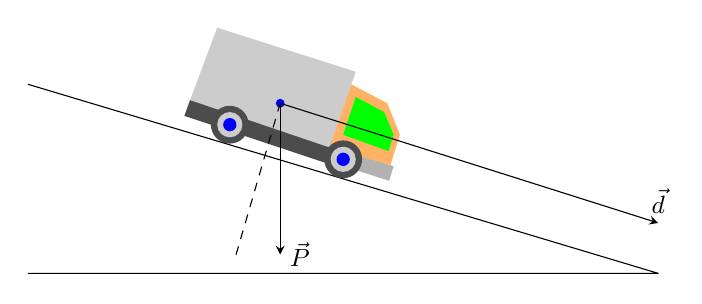
\begin{tikzpicture}[scale=0.8,font=\small, line join=round, line cap=round, >=stealth]
        \def\xe{orange!60}
        \def\den{red}
        \draw (0,3)--(10,0) (0,0)--(10,0);
        \fill[black!30] (2.48,2.5)--(2.57,2.75)--(5.8,1.7)--(5.73,1.47)--cycle ;
        \fill[black!70] (2.48,2.5)--(2.57,2.75)--(5.2,2)--(5.18,1.6)--cycle ;
        \fill[black!20] (2.57,2.75)--(3,3.9)--(5.2,3.2)--(4.78,2)--cycle ;
        \fill[\xe] (4.78,2)--(5.13,3)--(5.7,2.7)--(5.9,2.2)--(5.75,1.72)--cycle ;
        \fill[green] (5.2,2.8)--(5.65,2.56)--(5.8,2.2)--(5.72,1.94)--(5,2.2)--cycle ;
        \fill[black!70] (3.2,2.36) circle (0.3) (5,1.81) circle (0.3) ;
        \fill[black!20] (3.2,2.36) circle (0.2) (5,1.81) circle (0.2) ;
        \fill[blue](3.2,2.36) circle (3pt) (5,1.81) circle (3pt) (4,2.7) circle (2pt) ;
        \draw[dashed] (4,2.7)--(3.3,0.3) ;
        \draw[->] (4,2.7)--(4,0.3) node[right] {$\vec{P}$};
        \draw[->] (4,2.7)--(10,0.8) node[above] {$\vec{d}$};
    \end{tikzpicture}
}
Biết rằng trọng lực $\vec{P}$ được xác định bởi công thức $\vec{P} = m\vec{g}$, với $m$ (đơn vị: kg) là khối lượng của vật và $\vec{g}$ là gia tốc rơi tự do có độ lớn $g = 9{,}8$ m/s$^2$. Công sinh bởi trọng lực $\vec{P}$ khi xe đi hết đoạn đường dốc dài $7{,}5$ m là bao nhiêu KJ? (làm tròn kết quả đến hàng phần chục),
\shortans{$9\,6$}
    \loigiai{Ta có $1{,}5$ tấn = $1~500$ kg.\\
        Độ lớn của trọng lực tác dụng lên chiếc xe là $\left|\vec{P}\right| = m \left|\vec{g}\right| = 1~500\cdot 9{,}8 = 14~700$ (N).\\
        Vectơ $\vec{d}$ biểu thị độ dịch chuyển của xe có độ dài là $\left|\vec{d}\right| = 7{,}5$ (m) và $\left(\vec{P},\vec{d}\right)= 90^\circ - 5^\circ = 85^\circ$.\\
        Công sinh ra bởi trọng lực $\vec{P}$ khi xe đi hết đoạn đường dốc dài $30$ m là
        $$A=\vec{P}\cdot\vec{d}=\left|\vec{P}\right|\cdot\left|\vec{d}\right|\cdot\cos\left(\vec{P},\vec{d}\right) = 14~700\cdot 7{,}5\cdot \cos 85^\circ \approx 9\,609 \mathrm{\ (J)} =9{,}6 \mathrm{\ (KJ)}.$$
    }
    \dotlineEX{2}
\end{ex}

\begin{ex}%[2H2V1-4]
    \immini[thm]{Một chiếc ô tô được đặt trên mặt đáy dưới một khung sắt có dạng hình hộp chữ nhật với đáy trên là hình vuông $ABCD$, mặt phẳng $\left(ABCD\right)$ song song với mặt phẳng nằm ngang. Khung sắt đó được buộc vào móc $E$ của chiến cần cẩu sao cho các đoạn dây cáp $EA$, $EB$, $EC$, $ED$ có độ dài bằng nhau và cùng tạo với mặt phẳng $\left(ABCD\right)$ một góc $45^{\circ}$ như hình vẽ. Chiếc cần cẩu kéo khung sắt lên theo phương thẳng đứng. Biết lực căng $\left|\overrightarrow{F_1}\right|=\left|\overrightarrow{F_2}\right|=\left|\overrightarrow{F_3}\right|=\left|\overrightarrow{F_4}\right|$, trọng lượng khung sắt là $1\,000$ (N) và trọng lượng của chiếc xe ô tô là $4\,000$ (N). Tính cường độ lực căng của mỗi đoạn dây cáp (làm tròn đến hàng đơn vị).
    \shortans{$1768$}
    }{\begin{tikzpicture}[scale=0.6,>=latex,line join=round, line cap=round,scale=1,transform shape]
            \definecolor{bostonuniversityred}{rgb}{0.8, 0.0, 0.0}
            \definecolor{charcoal}{rgb}{0.21, 0.27, 0.31}
            \definecolor{bananayellow}{rgb}{1.0, 0.88, 0.21}
            \definecolor{anti-flashwhite}{rgb}{0.95, 0.95, 0.96}
            %	\clip (-6,-3) rectangle (6,3);
            \tikzset{%
            xeoto/.pic={%
                    %--------------------------
                    \tikzset{xe/.pic={
                            \def\N{
                                (-2.7,.56)--(-2.5,.56)
                                ..controls +(50:1.5) and +(165:1.5) .. (2.1,1.88)--(2.05,2)
                                ..controls +(-10:.1) and +(130:.1) .. (3.25,1.75)--(3.15,1.65)
                                ..controls +(-4:.2) and +(130:.15) .. (4.05,.7)--(4.25,.75)
                                ..controls +(-40:.2) and +(130:.15) .. (4.55,.35)--(4.35,.26)
                                ..controls +(-40:.2) and +(130:.15) .. (4.8,-.45)--(4.92,-.4)
                                ..controls +(-40:.25) and +(73:.17) .. (4.8,-1.8)--(-4.4,-1.8)
                                ..controls +(175:.7) and +(-175:3.2) ..cycle
                                ;
                            }
                            \fill[bostonuniversityred] \N;
                            \draw \N;
                            \def\K{
                                (-2.2,.56)--(3.3,.7)
                                ..controls +(100:1.18) and +(43:3) .. cycle
                                ;
                            }
                            \fill[bottom color=charcoal,top color=charcoal!20!white, middle color=charcoal!80!white] \K;
                            \draw \K;
                            \def\K1{
                                (-2.2,.56)
                                ..controls +(43:.2) and +(43:.2) .. (-1.58,1.05)--(-1.53,.57)--cycle
                                ;
                            }
                            \draw \K1;
                            \fill[charcoal] \K1;
                            \def\K2{
                                (1.2,1.85)
                                ..controls +(-10:.1) and +(160:.1) .. (1.58,1.8)--(1.8,.65)--(1.25,.65)--cycle
                                ;
                            }
                            \draw \K2;
                            \fill[charcoal] \K2;
                            \def\Kt{
                                (-2.5,.56)
                                ..controls +(50:1.5) and +(165:1.5) .. (2.1,1.88)--(2.05,2)
                                ..controls +(170:2.2) and +(45:1.5) .. (-2.7,.56)--cycle
                                ;
                            }
                            \fill[charcoal!50] \Kt;
                            \draw \Kt;
                            \def\Ks{
                                (3.25,1.75)--(3.15,1.65)
                                ..controls +(-4:.2) and +(130:.15) .. (4.05,.7)--(4.22,.75)
                                ..controls +(120:.3) and +(-35:.3) .. cycle
                                ;
                            }
                            \fill[charcoal!50] \Ks;
                            \draw \Ks;
                            %Đèn sau
                            \def\D{
                                (4.55,.35)--(4.35,.26)
                                ..controls +(-40:.2) and +(130:.15) .. (4.8,-.45)--(4.92,-.4)
                                ..controls +(110:.2) and +(-40:.15) ..cycle
                                ;
                            }
                            \fill[bananayellow] \D;
                            \draw \D;
                            \def\M{
                                (2.2,-1.3)--(-1.8,-1.4)--(-1.78,-1.7)
                                ..controls +(-5:.3) and +(-90:.6) ..cycle
                                ;
                            }
                            \draw \M;
                            \fill[charcoal!90] \M;
                            \draw (-1.6,.55)
                            ..controls +(-170:.5) and +(95:.4) .. (-1.78,-1.7)
                            (1.6,.65)
                            ..controls +(-30:.5) and +(35:.3) .. (1.7,-1.3)
                            ;
                            %gương
                            \def\G{
                                (-1.5,.45)--(-1.4,.6)
                                ..controls +(85:1) and +(20:.6) .. (-1.25,.5)--(-1.4,.33)
                                ;
                            }
                            \draw \G;
                            \fill[bostonuniversityred] \G;
                            %Đèn trước
                            \def\Dt{
                                (-4.85,-.7)
                                ..controls +(75:1) and +(65:.8) .. (-4.5,-.7)
                                ..controls +(-115:.6) and +(-105:.4) .. cycle
                                ;
                            }
                            \fill[bananayellow] \Dt;
                            \draw \Dt;
                            \def\Dt2{
                                (-4.85,-.7)
                                ..controls +(75:.6) and +(65:.4) .. (-4.7,-.7)
                                ..controls +(-115:.3) and +(-105:.2) .. cycle
                                ;
                            }
                            \fill[anti-flashwhite] \Dt2;
                            \draw \Dt2;
                            \draw[fill=anti-flashwhite] (-4.86,-1.45)--(-4.82,-1.5)--(-4.55,-1.3)
                            ..controls +(90:.3) and +(45:.2) .. cycle;
                        }}
            \tikzset{banh_xe/.pic={
                        \draw[fill=charcoal] (-3.25,-1.65) circle (1) ;
                        \draw[fill=anti-flashwhite] (-3.25,-1.65) circle (.7) ;
                        \draw[fill=charcoal] (-3.25,-1.65) circle (.4) ;
                    }}
            %----------------
            \path
            (0,0)pic[scale=1]{xe}(0,0)pic[scale=1]{banh_xe}(6.9,0)pic[scale=1]{banh_xe};
            %--------------------------------
            }}
            %%%%%%%%%%%%%%%%%%%
            \def\bc{4.25} % cạnh BC
            \def\ba{1.5} % cạnh BA
            \def\h{4} % đường cao
            \def\gocnghieng{90} % góc nghiêng
            \def\gocB{160} % góc B của đáy
            \coordinate (B1) at (0,0);
            \coordinate (A1) at (\gocB:\ba);
            \coordinate (C1) at (\bc,0.25);
            \coordinate (D1) at ($(C1)-(B1)+(A1)$);
            \coordinate[label=above left:$A$] (A) at ($(A1)+(\gocnghieng:\h)$);
            \coordinate[label=below left:$B$] (B) at ($(B1)-(A1)+(A)$);
            \coordinate[label=right:$C$] (C) at ($(C1)-(A1)+(A)$);
            \coordinate[label=above right:$D$] (D) at ($(D1)-(A1)+(A)$);
            \coordinate (E) at ($(A)!0.5!(C)+(\gocnghieng:\h)$);
            \coordinate (O) at ($(A)!0.5!(C)$);
            \path (O) node[below]{$O$};
            %------------
            \draw[->,blue,very thick] (E)--($(E)!0.4!(A)$) ;
            \draw[->,blue,very thick] (E)--($(E)!0.4!(B)$) ;
            \draw[->,blue,very thick] (E)--($(E)!0.4!(C)$) ;
            \draw[->,blue,very thick] (E)--($(E)!0.4!(D)$) ;
            \draw[dashed] (A)--(C) (B)--(D);
            \draw[dashed] (E)--(O);
            %------------
            \path (E) node[left=1mm]{$E$};
            \draw[blue,very thick] (A)--(B)--(C)--(D)--cycle
            (A1)--(A) (D1)--(D) (C1)--(C)
            (A)--(E)--(B) (C)--(E)--(D);
            \draw[fill=teal] (A1)--(B1)--(C1)--(D1)--cycle;
            \draw[fill=teal!30] (A1)--(B1)--(C1)--++(0,-0.3)--([yshift=-0.3cm]B1)--([yshift=-0.3cm]A1)--cycle;
            \foreach \diem in {A1,B1,C1,D1,A,B,C,D,E}	\fill (\diem)circle(1.5pt);
            %phần móc và dây
            \def\r{0.3}\def\rr{0.25}
            \coordinate (tam) at ([yshift=6mm]E);
            \draw[brown,fill=brown,line width=1pt] (tam) circle (\r cm);
            \fill (tam) circle (2pt);
            \draw[brown,line width=1pt] (tam)++(\r,0)--++(0,0.7)
            (tam)++(-\r,0)--++(0,0.7);
            \draw[line width=1.5pt] (tam)--++(0,-1.35*\r) arc(90:370:1mm);
            %%%%%%%%%%%%%%%%%%%
            \pic[scale=0.45,rotate=4] at (1.6,1.3) [pic type = xeoto];
            %--------
            \draw[blue,very thick] (B)--(B1);
        \end{tikzpicture}}
    \par
    
    \loigiai{
        \begin{center}
            \begin{tikzpicture}[declare function={r=4;goc=18;},scale=1, line join=round, line cap=round, >=stealth, font=\small]
                \path (0:0) coordinate (O)
                (0:r) arc (0:goc:{r} and {0.35*r}) coordinate (A)
                arc (goc:goc+90:{r} and {0.35*r}) coordinate (B)
                arc (goc+90:goc+180:{r} and {0.35*r}) coordinate (C)
                arc (goc+180:goc+270:{r} and {0.35*r}) coordinate (D)
                (O)+(90:{0.95*r}) coordinate (E)
                (O)+(-90:{0.95*r}) coordinate (F)
                ($(A)!0.5!(E)$) coordinate (G)
                ($(B)!0.5!(E)$) coordinate (H)
                ($(C)!0.5!(E)$) coordinate (I)
                ($(D)!0.5!(E)$) coordinate (K)
                ;
                \draw[dashed](E)--(F) (A)--(C) (B)--(D)
                (A)--(B)--(C) (E)--(B)--(F);
                \draw[->] (E)--(I)node[above left]{$\overrightarrow{F}_1$};
                \draw[->] (E)--(G)node[above right]{$\overrightarrow{F}_2$};
                \draw[->] (E)--(H)node[below right]{$\overrightarrow{F}_3$};
                \draw[->] (E)--(K)node[above right]{$\overrightarrow{F}_4$};
                \draw (E)--(A)--(F) (E)--(C)--(F) (E)--(D)--(F)(C)--(D)--(A);
                \foreach \x in {A,B,C,D,O,E,F}\draw[fill=white] (\x) circle (1pt);
                \foreach \x/\goc/\t in {A/0/C,B/120/B,C/150/A,D/-30/D,E/90/E,F/-90/E',O/60/O}
                \draw[fill=white] (\x) circle (1pt) node[shift={(\goc:7pt)},font=\scriptsize]{$\t$};
            \end{tikzpicture}
        \end{center}
        Gọi $O$ là giao của hai đường chéo $AC$ và $BD$.\\
        Hình chóp $E.ABCD$ là chóp có các cạnh bên bằng nhau và $O$ là tâm của đáy là hình chữ nhật $ABCD$.Suy ra $EO\perp \left(ABCD\right)$.\\
        Ta có $\overrightarrow{F_1}=k\overrightarrow{EA}$; $\overrightarrow{F_2}=k\overrightarrow{EB}$; $\overrightarrow{F_3}=k\overrightarrow{EC}$; $\overrightarrow{F_4}=k\overrightarrow{ED}$.\\
        Lấy $E'$ đối xứng với $E$ qua $O$.\\
        Áp dụng quy tắc hình bình hành ta có $\overrightarrow{F_1}+\overrightarrow{F_3}=k\overrightarrow{EE^{'}}$; $\overrightarrow{F_2}+\overrightarrow{F_4}=k\overrightarrow{EE^{'}}$ (k là hằng số)
        $$\overrightarrow{F_1}+\overrightarrow{F_2}+\overrightarrow{F_2}+\overrightarrow{F_4}=2k\overrightarrow{EE^{'}}=4k\overrightarrow{EO}.
        $$
        Vì ô tô được đặt ở vị trí cân bằng nên $\overrightarrow{F_1}+\overrightarrow{F_2}+\overrightarrow{F_2}+\overrightarrow{F_4}=\overrightarrow{P}$, trong đó $\overrightarrow{P}$ là trọng lực tác dụng lên ô tô và khung sắt nên.
        $$5\,000=4kOE\Rightarrow OE=\dfrac{5\,000}{4k}=\dfrac{1\,250}{k} \quad(N).
        $$
        Vì $EA$ tạo với $\left(ABCD\right)$ một góc $45^\circ\Rightarrow \widehat{EAO}=45^\circ$.\\
        Xét $\triangle AEO$ vuông tại $O$ ta có $EO=AE\cdot\sin 45^\circ\Rightarrow \dfrac{1\,250}{k}=AE\cdot\dfrac{\sqrt{2}}{2} \Rightarrow AE=1\,250k\sqrt{2} \quad(N)$.\\
        Từ giả thiết $EA=EB=EC=ED=k\left|\overrightarrow{F_1}\right|$.\\
        Vậy cường độ lực căng của mỗi đoạn dây cáp là$\left|\overrightarrow{F_1}\right|=\dfrac{EA}{k}=\dfrac{1\,250k\sqrt{2}}{k}\quad (N)\approx 1\,768\quad(N)$.
    }
    \dotlineEX{4}
\end{ex}

\begin{ex}%[2H2V1-4]
\immini[thm]
{
    Trong không gian với hệ trục tọa độ $Oxyz$,một tấm bảng đồng chất có dạng hình vuông $ABCD$ tâm $O$ được treo nghiêng bởi $4$ sợi dây $IA$, $IB$, $IC$, $ID$ gắn cố định tại điểm $I(0;0;9)$ như hình vẽ. Điểm $O(0;0;5)$; $A(-\sqrt{2};\sqrt{2};5)$ và góc $\widehat{OID}$ đạt giá trị lớn nhất. Gọi $\overrightarrow{F}_1$, $\overrightarrow{F}_2$, $\overrightarrow{F}_3$, $\overrightarrow{F}_4$ lần lượt là lực căng của các sợi dây $IB$, $IC$, $ID$, $IA$. Biết rằng $\left|\overrightarrow{F}_1\right| = 50\,\text{N}$ và $\left|\overrightarrow{F}_2\right| = 40\,\text{N}$.
    Tính khối lượng $m$ (kg) của tấm bảng (Kết quả làm tròn đến hàng đơn vị) (Cho gia tốc trọng trường $g = 9,8 \, (\text{m/s}^2)$ và trọng lượng của tấm bảng được tính bằng công thức $P = m \cdot g$).
    \shortans[0]{15}
}
{
    \begin{tikzpicture}[scale=0.7, font=\small, line join=round,line cap=round, >=stealth,thick]
        \path
        (0,0) coordinate (A)
        (A)+(10:5) coordinate (D)
        (A)+(-150:3) coordinate (B)
        ($(B)+(D)-(A)$) coordinate (C)
        ($(A)!.5!(C)$) coordinate (O)
        (O)+(90:5) coordinate (S)
        ;
        \draw[dashed,thin] (D)--(A)--(B) (S)--(A)--(C) (B)--(D) (S)--(O);
        \draw (D)--(C)--(B)--(S)--(C) (S)--(D);
        \foreach \i/\g in {A/180,B/-90,C/-90,D/0,O/-90,S/90} \fill (\i) circle(1pt) + (\g:0.4) node{$\i$};
        \draw[->,red] (S)--($(S)!1/3!(B)$) node[sloped,pos=0.5,above] {$\overrightarrow{F_1}$};
        \draw[->,red] (S)--($(S)!1/3!(D)$) node[sloped,pos=0.5,above] {$\overrightarrow{F_3}$};
    \end{tikzpicture}
}
    \loigiai{
        \begin{center}
            \begin{tikzpicture}[scale=0.7, font=\small, line join=round,line cap=round, >=stealth,thick]
                \path
                (0,0) coordinate (A)
                (A)+(10:5) coordinate (D)
                (A)+(-150:3) coordinate (B)
                ($(B)+(D)-(A)$) coordinate (C)
                ($(A)!.5!(C)$) coordinate (O)
                (O)+(90:5) coordinate (S)
                ;
                \draw[dashed,thin] (D)--(A)--(B) (S)--(A)--(C) (B)--(D) (S)--(O);
                \draw (D)--(C)--(B)--(S)--(C) (S)--(D);
                \foreach \i/\g in {A/180,B/-90,C/-90,D/0,O/-90,S/90} \fill (\i) circle(1pt) + (\g:0.4) node{$\i$};
                \draw[->,red] (S)--($(S)!1/3!(B)$) node[sloped,pos=0.5,above] {$\overrightarrow{F_1}$};
                \draw[->,red] (S)--($(S)!1/3!(D)$) node[sloped,pos=0.5,above] {$\overrightarrow{F_3}$};
            \end{tikzpicture}
        \end{center}
        Do $O$ là trung điểm của $AC$ nên $C(\sqrt{2};-\sqrt{2};5)$ và gọi $D(a;b;c)$.\\
        Khi đó $\overrightarrow{OD} = (a;b;c-5)$; $\overrightarrow{AC} = (2\sqrt{2}; -2\sqrt{2}; 0)$ mà hai vectơ này vuông góc với nhau.\\
        Từ đó $2\sqrt{2}a = 2\sqrt{2}b \Rightarrow a=b \Rightarrow \overrightarrow{DC} = (a-\sqrt{2}; a+\sqrt{2}; c-5)$; $\overrightarrow{DA} = (a+\sqrt{2}; a-\sqrt{2}; c-5)$.\\
        Ta có $\overrightarrow{ID} = (a; a; \sqrt{4-2a^2}-4)$; $\overrightarrow{IO} = (0;0;-4) \Rightarrow \cos \widehat{OID} = \dfrac{16-4\sqrt{4-2a^2}}{16\sqrt{a^2+a^2+(4-\sqrt{4-2a^2})^2}}$.\\
        Khảo sát hàm số $f(a) = \dfrac{16-4\sqrt{4-2a^2}}{16\sqrt{a^2+a^2+(4-4\sqrt{4-2a^2})^2}}$ tìm được $a = \dfrac{\sqrt{6}}{2}$.\\
        Vậy tọa độ các điểm $A(-\sqrt{2};\sqrt{2};5)$; $B\left(-\dfrac{\sqrt{6}}{2};-\dfrac{\sqrt{6}}{2};1\right)$; $C(\sqrt{2};-\sqrt{2};5)$; $D\left(\dfrac{\sqrt{6}}{2};\dfrac{\sqrt{6}}{2};6\right)$.\\
        Ta có $\overrightarrow{IA}=(-\sqrt{2};\sqrt{2};-4) \Rightarrow \left|\overrightarrow{IA}\right|=2\sqrt{5}$; $\overrightarrow{IC}=(\sqrt{2};-\sqrt{2};-4) \Rightarrow \left|\overrightarrow{IC}\right|=2\sqrt{5}$.\\
        Vậy $\left|\overrightarrow{F}_4\right|=\left|\overrightarrow{F}_2\right|=k \cdot 2\sqrt{5} = 40 \Rightarrow k=4\sqrt{5}$.\\
        Suy ra $\overrightarrow{F}_2 = (-4\sqrt{10}; 4\sqrt{10}; -16\sqrt{5})$; $\overrightarrow{F}_4 = (4\sqrt{10}; -4\sqrt{10}; -16\sqrt{5})$.\\
        Tương tự $\overrightarrow{IB}=\left(-\dfrac{\sqrt{6}}{2};-\dfrac{\sqrt{6}}{2};-5\right) \Rightarrow \left|\overrightarrow{IB}\right|=2\sqrt{7}$; $\overrightarrow{ID}=\left(\dfrac{\sqrt{6}}{2};\dfrac{\sqrt{6}}{2};-3\right) \Rightarrow \left|\overrightarrow{ID}\right|=2\sqrt{3}$.\\
        Sử dụng tỉ lệ giữa độ dài dây và độ lớn lực: $\dfrac{\left|\overrightarrow{F}_1\right|}{\left|\overrightarrow{F}_3\right|} = \dfrac{2\sqrt{7}}{2\sqrt{3}} \Rightarrow \left|\overrightarrow{F}_3\right| = \dfrac{50\sqrt{21}}{7}$.\\
        Suy ra $\overrightarrow{F}_3 = \left(\dfrac{25\sqrt{42}}{14}; \dfrac{25\sqrt{42}}{14}; -\dfrac{75\sqrt{7}}{7}\right)$; $\overrightarrow{F}_1 = \left(-\dfrac{25\sqrt{42}}{14}; -\dfrac{25\sqrt{42}}{14}; -\dfrac{125\sqrt{7}}{7}\right)$.\\
        Để hệ cân bằng thì $\overrightarrow{F}_1+\overrightarrow{F}_2+\overrightarrow{F}_3+\overrightarrow{F}_4=\overrightarrow{P}=\left(0;0;-32\sqrt{5}-\dfrac{200\sqrt{7}}{7}\right) \Rightarrow \left|P\right|=\dfrac{200\sqrt{7}}{7}+32\sqrt{5}$.\\
        Vậy khối lượng của thanh kim loại là $m=\dfrac{P}{g}=\dfrac{\dfrac{200\sqrt{7}}{7}+32\sqrt{5}}{9,8} \approx 15{,}015 \approx 15 \, (\text{kg})$
    }
\end{ex}
\Closesolutionfile{ans}
%\inputansbox{5}{ans/DA-CD3-BTRL}